%% 
%% Copyright 2007, 2008, 2009 Elsevier Ltd
%% 
%% This file is part of the 'Elsarticle Bundle'.
%% ---------------------------------------------
%% 
%% It may be distributed under the conditions of the LaTeX Project Public
%% License, either version 1.2 of this license or (at your option) any
%% later version.  The latest version of this license is in
%%    http://www.latex-project.org/lppl.txt
%% and version 1.2 or later is part of all distributions of LaTeX
%% version 1999/12/01 or later.
%% 
%% The list of all files belonging to the 'Elsarticle Bundle' is
%% given in the file `manifest.txt'.
%% 
%% Template article for Elsevier's document class `elsarticle'
%% with harvard style bibliographic references
%% SP 2008/03/01

%\documentclass[preprint,12pt,authoryear]{elsarticle}  %default in the template
%\documentclass[preprint,10pt,authoryear]{elsarticle}

%% Use the option review to obtain double line spacing
%% \documentclass[authoryear,preprint,review,12pt]{elsarticle}

%% Use the options 1p,twocolumn; 3p; 3p,twocolumn; 5p; or 5p,twocolumn
%% for a journal layout:
%% \documentclass[final,1p,times,authoryear]{elsarticle}
%% \documentclass[final,1p,times,twocolumn,authoryear]{elsarticle}
 \documentclass[final,3p,times,authoryear]{elsarticle}
%% \documentclass[final,3p,times,twocolumn,authoryear]{elsarticle}
%% \documentclass[final,5p,times,authoryear]{elsarticle}
%% \documentclass[final,5p,times,twocolumn,authoryear]{elsarticle}

%% For including figures, graphicx.sty has been loaded in
%% elsarticle.cls. If you prefer to use the old commands
%% please give \usepackage{epsfig}

%% The amssymb package provides various useful mathematical symbols
\usepackage{amssymb}
%% The amsthm package provides extended theorem environments
 \usepackage{amsthm}
 \usepackage{amsmath}
 \usepackage{color}
 \usepackage{amsmath}
\usepackage{siunitx}


\usepackage{framed} % Framing content
\usepackage{multicol} % Multiple columns environment
\usepackage{nomencl} % Nomenclature package
\makenomenclature
%\setlength{\nomitemsep}{-\parskip} % Baseline skip between items
\setlength{\nomitemsep}{0.01cm}
\renewcommand*\nompreamble{\begin{multicols}{2}}
\renewcommand*\nompostamble{\end{multicols}}


%% The lineno packages adds line numbers. Start line numbering with
%% \begin{linenumbers}, end it with \end{linenumbers}. Or switch it on
%% for the whole article with \linenumbers.
%% \usepackage{lineno}

\journal{Urban Climate}

\begin{document}

\begin{frontmatter}

%% Title, authors and addresses

%% use the tnoteref command within \title for footnotes;
%% use the tnotetext command for theassociated footnote;
%% use the fnref command within \author or \address for footnotes;
%% use the fntext command for theassociated footnote;
%% use the corref command within \author for corresponding author footnotes;
%% use the cortext command for theassociated footnote;
%% use the ead command for the email address,
%% and the form \ead[url] for the home page:
%% \title{Title\tnoteref{label1}}
%% \tnotetext[label1]{}
%% \author{Name\corref{cor1}\fnref{label2}}
%% \ead{email address}
%% \ead[url]{home page}
%% \fntext[label2]{}
%% \cortext[cor1]{}
%% \address{Address\fnref{label3}}
%% \fntext[label3]{}

\title{Development of the VTUF-3D v1.0 urban micro-climate model to support assessments of urban vegetation influences on HTC}


%% use optional labels to link authors explicitly to addresses:
\author[monash,crc]{Kerry~A~Nice\corref{cor1}}
\ead{mothlight@fastmail.fm}
\author[monash,crc]{Andrew Coutts}
\author[monash,crc]{Nigel~Tapper}
\cortext[cor1]{Principal corresponding author}
\address[monash]{School of Earth, Atmosphere and Environment, Monash University, Clayton, VIC 3800, Australia}
\address[crc]{CRC for Water Sensitive Cities, Australia}


\begin{abstract}

With urban areas facing future longer duration heat-waves and temperature extremes from climate change and growing urban development, adaptation strategies are needed to protect city residents. Examining the role that increased tree cover and water availability can have on human thermal comfort (HTC) is needed to help guide the development of thermally comfortable cities. To inform planning, modelling tools are needed that provide sufficient resolution to resolve urban influences on HTC and the ability to model important physiological processes of vegetation. A new micro-scale model, VTUF-3D (Vegetated Temperatures Of Urban Facets), has been developed to achieve this, by embedding the functionality of the MAESPA tree process model \citep{Duursma2012}, that can model individual trees, vegetation, and soil components, within the TUF-3D \citep{Krayenhoff2007} urban micro-climate model. An innovative tiling approach allows the new model to account for important vegetative physiological processes and shading effects, using configurable templates to allow representation of any type of vegetation or water sensitive design feature. This allows detailed calculations of surface temperatures ($T_{sfc}$), mean radiant temperature ($T_{mrt}$), and a HTC index, the universal thermal climate index (UTCI), across an urban canyon. This study presents an outline of VTUF-3D, along with a validation of the modelled surface energy balance for Preston, Australia \citep{Coutts2007}. The VTUF-3D model has shown it performs well and is suitable for use to examine critical questions relating to the role of vegetation and water in the urban environment. Using this model, it is now possible to conduct further analysis to quantify the impact each individual tree can have on temperatures in urban canyons. Further, the model can help inform the optimal arrangement and quantity of trees to maximise temperature moderation effects and be used to generate best practices guidelines for urban greening.

\nomenclature{$T_{mrt}$}{mean radiant temperature (\SI{}{\degreeCelsius})}  
\nomenclature{$UTCI$}{universal thermal climate index}
\end{abstract}

\begin{keyword}
micro-climate modelling, urban vegetation, VTUF-3D
%% keywords here, in the form: keyword \sep keyword

%% PACS codes here, in the form: \PACS code \sep code

%% MSC codes here, in the form: \MSC code \sep code
%% or \MSC[2008] code \sep code (2000 is the default)

\end{keyword}

\end{frontmatter}

\begin{table*}[!t]   
\begin{framed}
\printnomenclature
%%\nomenclature{$A _{canopy}$}{canopy area (m$^{2}$)} 
%\nomenclature{$A _{mm}$}{2-dimensional tree area (mm$^{2}$)} 
%\nomenclature{$A$}{surface area of a sphere of diameter D, of value 0.15m, (=$\pi 0.15^{2}$m$^{2}$)} 
%\nomenclature{$A_{leaf}$}{total leaf area (m$^{2}$)} 
%%\nomenclature{$D_{eff}$}{effective diffusivity of the soil pore space (m$^{2}$s$^{-1}$)} 
%%\nomenclature{$E_{L}$}{leaf level transpiration rate ($\mu$mol m$^{-2}$s$^{-1}$)} 
%%\nomenclature{$E_{i}$}{root water uptake (canopy transpiration) out of layer i (mm)} 
%%\nomenclature{$E_{s}$}{rate of evaporation (mm)} 
%%\nomenclature{$F_{R}$}{cumulative fraction of fine roots to depth z (m)} 
%%\nomenclature{$G_{ws}$}{conductance of water vapour through the soil pore space (m s$^{-1}$)} 
%\nomenclature{$H _{blt}$}{building height (m)} 
%\nomenclature{$H _{crown}$}{crown height (m)} 
%\nomenclature{$H _{trunk}$}{trunk height (m)} 
%\nomenclature{$H$}{tree height (m)}
%\nomenclature{$H_{top}$}{convective sensible heat flux density between canopy air and boundary layer (Wm$^{-2}$)} 
%%\nomenclature{$K\downarrow$}{downward shortwave radiative flux density (Wm$^{-2}$)} 
%\nomenclature{$K\downarrow_{dir,i}$}{incident direct shortwave (Wm$^{-2}$)}  
%\nomenclature{$L \downarrow_{i,sky}$}{initial incident sky-derived longwave (Wm$^{-2}$)}  
%\nomenclature{$LAI$}{leaf area index (m$^{2}$m$^{-2}$)} 
%%\nomenclature{$L\downarrow$}{downward longwave radiative flux density (Wm$^{-2}$)}
%\nomenclature{$L\uparrow$}{upward longwave radiative flux density (Wm$^{-2}$)} 
%\nomenclature{$Nu$}{Nusselt number (-)} 
%\nomenclature{$P_{o}$}{vapour pressure of water at infinite temperature (=7.5152 $\times$ 10$^8$ mb)} 
%\nomenclature{$Pr$}{Prandtl number (-)} 
%%\nomenclature{$Q^{*}$}{net radiation flux density (Wm$^{-2}$)} 
%%\nomenclature{$Q^{*}_{veg}$}{calculation of vegetation net radiation flux density (Wm$^{-2}$)}
%\nomenclature{$Q_{E,canopy}$}{latent heat flux calculated from $canopystore$ (Wm$^{-2}$)} 
%\nomenclature{$Q_{E,et}$}{latent heat flux calculated from $et$ (Wm$^{-2}$)} 
%\nomenclature{$Q_{E,evap}$}{latent heat flux calculated from $evapstore$ (Wm$^{-2}$)} 
%\nomenclature{$Q_{E,soil}$}{latent heat flux calculated from $soilstore$ (Wm$^{-2}$)} 
%%\nomenclature{$Q_{E,veg}$}{calculation of vegetation latent heat flux (Wm$^{-2}$)} 
%%\nomenclature{$Q_{E}$}{latent heat flux (Wm$^{-2}$)}
%%\nomenclature{$Q_{G,street}$}{calculation of street ground heat storage (Wm$^{-2}$)} 
%%\nomenclature{$Q_{G,veg}$}{calculation of vegetation ground heat storage (Wm$^{-2}$)} 
%%\nomenclature{$Q_{G}$}{ground heat storage (Wm$^{-2}$)} 
%%\nomenclature{$Q_{H,veg}$}{calculation of vegetation sensible heat flux (Wm$^{-2}$)} 
%%\nomenclature{$Q_{H}$}{sensible heat flux (Wm$^{-2}$)} 
%\nomenclature{$Re$}{Reynolds number (-)} 
%\nomenclature{$S$}{horizontal solar irradiance (Wm$^{-2}$)}  
%\nomenclature{$S^{*}$}{$S^{*} = S/S_{max}$}
%\nomenclature{$S_{0}$}{solar constant (=1367 Wm$^{-2}$)} 
%\nomenclature{$T$}{temperature (K)} 
%%\nomenclature{$T(z)$}{air temperature at height z (K)} 
%%\nomenclature{$T_{1}$}{temperature of the shallowest layer (K)} 
%\nomenclature{$T_{a}$}{dry bulb air temperature (K)} 
%%\nomenclature{$T_{can}$}{canopy air temperature ($z < z_{H}$) (K)} 
%%\nomenclature{$T_{conv}$}{converging canyon temperature (K)} 
%%\nomenclature{$T_{g}$}{globe temperature (K)} 
%\nomenclature{$T_{mrt}$}{mean radiant temperature (\SI{}{\degreeCelsius})}  
%%\nomenclature{$T_{m}$}{temperature of the deepest layer (K)} 
%\nomenclature{$T_{sfc,i}$}{surface temperature of patch i (K)} 
%%\nomenclature{$T_{sfc,veg}$}{vegetation surface temperature (K)} 
%%\nomenclature{$T_{sfc}$}{surface temperature (K)} 
%%\nomenclature{$U(z)$}{wind speed at height z (m s$^{-1}$)}  
%\nomenclature{$UTCI$}{universal thermal climate index}
%%\nomenclature{$U_{eff}(z)$}{effective wind speed at height z (m s$^{-1}$)} 
%%\nomenclature{$W_{i}$}{water storage of the layer i (mm)} 
%\nomenclature{$\Delta H_{vap}$}{enthalpy of evaporation (=42809 J mol$^{-1}$)} 
%%\nomenclature{$\Psi_{L}$}{leaf water potential (MPa)} 
%%\nomenclature{$\alpha _{veg}$}{shortwave albedo of vegetation}
%%\nomenclature{$\alpha$}{shortwave albedo }
%\nomenclature{$\alpha_{g}$}{globe albedo (=0.05)} 
%\nomenclature{$\alpha_{sfc}$}{surface albedo (=0.15)} 
%\nomenclature{$\delta{A}$}{change in rate of assimilation (mol m$^{-2}$s$^{-1}$)} 
%\nomenclature{$\delta{E}$}{change in the rate of transpiration per unit area of leaf (mol m$^{-2}$s$^{-1}$)}
%%\nomenclature{$\epsilon _{veg}$}{longwave emissivity of vegetation}
%%\nomenclature{$\epsilon$}{longwave emissivity}
%\nomenclature{$\epsilon_{a}$}{longwave emissivity of the atmosphere} 
%\nomenclature{$\epsilon_{g}$}{globe emissivity (=0.95)}  
%%\nomenclature{$\sigma$}{Stefan-Boltzmann constant (=5.67 $\times$ 10$^{-8}$Wm$^{-2}$K$^{-4}$)} 
%\nomenclature{$\theta$}{solar zenith angle} 
%\nomenclature{$c_{w,kj}$}{conversion to watts (=1W/1000KJ/sec)} 
%\nomenclature{$d$}{earth-sun distance (=1 A.U.)} 
%\nomenclature{$diam _{stem}$}{stem diameter (m)} 
%\nomenclature{$e_{a}$}{partial water vapour pressure of the air (KPa)} 
%%\nomenclature{$e_{s}$}{partial water vapour pressure of the soil pore space (KPa)} 
%\nomenclature{$et$}{evapotranspiration (mm)} 
%\nomenclature{$f_{dir}$}{fraction of the total horizontal solar irradiance, $S$, due to the direct }
%%\nomenclature{$g_{B}$}{boundary layer conductance (mol m$^{-2}$s$^{-1}$)} 
%%\nomenclature{$g_{V}$}{total conductance to water vapour (mol m$^{-2}$s$^{-1}$)} 
%\nomenclature{$g_{s}$}{leaf-level stomatal conductance to CO$_{2}$ (mol m$^{-2}$s$^{-1}$)} 
%%\nomenclature{$h$}{convective heat transfer coefficient (Wm$^{-2}$K$^{-1}$)} 
%%\nomenclature{$h_{i}$}{heat transfer coefficient (Wm$^{-2}$K$^{-1}$)} 
%\nomenclature{$k$}{thermal conductivity of the fluid (i.e. air) (Wm$^{-1}$ K$^{-1}$)} 
%\nomenclature{$k_{1}$}{thermal conductivity of the surface (Wm$^{-1}$K$^{-1}$)} 
%%\nomenclature{$k_{L}$}{total leaf-specific hydraulic conductance (mmol m$^{-2}$s$^{-1}$MPa$^{-1}$)} 
%\nomenclature{$l_{p}$}{length of a patch side (m)} 
%\nomenclature{$m_{mol,w}$}{molar mass of water (=18.0152 g mol$^{-1}$)} 
%\nomenclature{$n _{hts}$}{number of building heights} 
%\nomenclature{$n _{roofs}$}{number of roofs} 
%\nomenclature{$r _{xcrown}$}{crown radius in x direction (m)} 
%\nomenclature{$r _{ycrown}$}{crown radius in y direction (m)} 
%%\nomenclature{$r_{w,i}$}{wall roughness coefficient of patch i} 
%\nomenclature{$ws$}{wind speed (m s$^{-1}$)} 
%\nomenclature{$ws_{cm}$}{wind speed (cm s$^{-1}$)} 
%\nomenclature{$z_{0,Ht}$}{roughness length (m)} 
%\nomenclature{$z_{Ht}$}{measurement height of wind speed (m)} 
%\nomenclature{$z_{H}$}{mean building height (m)} 
%\nomenclature{$z_{PD}$}{zero-plane displacement height (m)} 
%%\nomenclature{$z_{horz,i}$}{height of patch forcing U(z) and T(z) above street level of patch i (m)} 
%%\nomenclature{$z_{i}$}{depth to the bottom of layer i (m)} 
\end{framed}
\end{table*}



%% \linenumbers

%% main text

\section{Introduction}\label{sec:introduction}
Urban areas are facing a growing number of challenges. Cities are now home to the majority of the world's population and trends will result in further increases \citep{UNDESA2015,WHO2016}. To accommodate increasing urban populations \citep{ABS2008}, cities are expanding \citep{Seto2011} and densifying \citep{Byrne2016,Ruth2016,DSE2002}, leading to loss of urban green spaces \citep{Hamin2009,Coutts2007}. In these increasingly urbanised areas, the removal of vegetation, combined with rapid stormwater removal, and possibly restricted irrigation during drought conditions, can leave urban landscape water starved. Urban development that does not consider the implications on urban climate, risks intensifying urban heating and compromising the thermal comfort of city residents. In addition, climate trends are towards increased average temperatures and increasing temperature extremes \citep{Alexander2009,IPCC2013a}. This is concerning given the increasing understanding of the impacts on human health of extreme temperatures \citep{Katsouyanni1993,Nicholls2008,Loughnan2010} and demographics that are shifting towards increased older and elderly citizens \citep{Cohen2003,FIFARS2016} that are particularly vulnerable to extreme heat. These factors leave those in urban areas in an increasingly dangerous position. In coming years, strategies are needed to adapt to and deal with these challenges.

Incorporating more vegetation and water into urban areas can be an effective way to mitigate extreme urban temperatures. From an examination of a range of different studies exploring cooling effects of urban greenery \citep{Tsiros2010,Shashua-Bar2010a,Spangenberg2008}, it is clear that increased vegetation and water can have positive benefits, from city-wide scale down to a micro-climate street level scale \citep{Coutts2012}. Shading and evapotranspiration are cited as the main drivers of these cooling effects \citep{Bowler2010}. The degree of cooling effects are variable however, and depend on factors such as vegetation density \citep{Hall2016,Bodnaruk2017}, street orientation and aspect ratio \citep{Thorsson2011,Ali-Toudert2006b}, and amounts of irrigation used \citep{Jenerette2011}. Trees in particular provide a strong benefit for HTC during the day, especially those with large, dense canopies that provide shade and are well irrigated to promote transpiration \citep{Coutts2015,Huang2008,Ylmaz2007,Shashua-Bar2000}. Water sensitive urban design (WSUD) presents an opportunity to capture and retain stormwater in urban areas using engineered and natural features (trees and vegetation) to capture, filter, and store water as an additional urban water source \citep{Wong2009}. A more focused effort in using trees and WSUD for urban climate benefits can deliver improvements to human thermal comfort (HTC) \citep{Coutts2012}. 


While the benefits of urban vegetation and water are well understood in the climate community, uptake and application of knowledge in urban planning is lacking. Yet, \cite{Bowler2010} suggests that the current research does not demonstrate exactly how urban greening should be implemented in terms of abundance, type and distribution.  A suitable modelling tool is needed to provide solid quantitative assessments of the effectiveness of trees and water in terms of heat mitigation, across contrasting micro-scale urban environments and therefore provide guidance on how to most effectively use trees and WSUD for improved HTC. 

A suitable modelling tool for these assessments needs to resolve detailed temperature gradients (as well as wind speed and humidity in order to calculate HTC) across a modelled urban canyon. This necessitates micro-scaled resolution climate modelling. In addition, modelling needs to incorporate important cooling mechanisms of evapotranspiration and shading. This requires proper modelling of vegetation, including vegetation physiology to estimate accurate latent energy fluxes and the soil-vegetation-atmosphere pathway critical for vegetation and WSUD assessments within the urban canyon. Models such as SOLWEIG \citep{SOLWEIG2011} and RayMan \citep{Matzarakis2007,Matzarakis2010} resolve at a suitable scale and generate useful insights into mean radiant temperatures in urban areas \citep{Chen2014a}, however they only capture the radiation shading effects of vegetation, and are unable to account for the effects of water and evapotranspiration. At the other end of the complexity spectrum, a number of models, primarily based on computational fluid dynamics (CFD), are able to resolve at a micro-scale and account for many of the influences of vegetation \citep{Bailey2014,Bailey2016,Kunz2000,Schlunzen2011a,Yamada2011,Bruse1999}. However their complexity and computational intensity leaves them out of reach for less specialised users.


What is needed is an approach that fits in between these two levels of complexity, a new innovative method to balance detail, accuracy, and complexity with efficiency and usability, while also being able to consider a wide variety of vegetation types and arrangements. This approach needs to capture the detailed movement of radiation through complex urban areas integrated with a widely configurable amount of vegetation. It also needs to balance this complexity against usability to create a model that can be widely used to consider a large variety of questions about HTC impacts of urban vegetation in support of urban planning decisions and guidelines. This study presents the development of a new model: VTUF-3D (Vegetated Temperatures of Urban Facets in 3D v1.0) that aims to provide a model capable of assessing the benefits of vegetation (including trees) and WSUD on urban canopy layer air temperature and HTC. VTUF-3D is developed from the TUF-3D (Temperatures Of Urban Facets in 3D) model \citep{Krayenhoff2007} that prior to this study, lacked vegetation and water components. The TUF-3D was coupled with the MAESPA model \citep{Duursma2012}, allowing insertion of any type of vegetation in any arrangement, accounting for vegetation structural and physiological processes. This study also aims to evaluate the model, in terms of the surface energy balance, for an urban site in Melbourne, Australia.

VTUF-3D has the capacity to address the research gap identified by \cite{Bowler2010} around identifying how vegetation (especially trees) should be implemented in terms of abundance, type and distribution, as well as the potential for accounting for water availability through WSUD. This can facilitate the integration of urban greening into the urban landscapes and inform planning decisions, with urban climate knowledge, about how to best utilise urban greening to maximise the thermal comfort impacts and meet the challenges of urban heat. VTUF-3D can help inform how to best to protect human health in light of all the concerning trends progressing in urban areas.

\section{Model design}\label{sec:method}

\subsection{Overview of the VTUF-3D model}\label{sec:DesignOverview}

To model the impacts of increased water and vegetation on human thermal comfort in urban areas requires modifications to the TUF-3D \citep{Krayenhoff2007} model. TUF-3D in its unmodified form lacks functionality for the physical representation of vegetation along with their physiological processes. Also missing are latent energy fluxes and the water cycle associated with soil, vegetation, evaporation, and precipitation. 

Two major changes were made to the TUF-3D model to add this missing functionality. The first is the representation of the physical form of vegetation and the associated radiative interactions within an urban canyon. VTUF-3D uses cube shaped structures (as TUF-3D uses to represent buildings) to represent vegetation. A single tower of cubes forms the tree trunk at the x,y location of the tree and extends upward to the height of the tree. If a canopy extends past the surface grid square boundaries, additional cubes are allowed to overhang the ground surface to fill out the full width of the canopy. These cubes store the surface properties and states and interact with the rest of the VTUF-3D domain. The vegetation’s true shape (e.g. ellipsoidal, conical, etc.) is represented in MAESPA \citep{Duursma2012}, with each vegetation element individually modelled offline, calculating values of vegetation absorption, transmission, and reflection to be loaded by VTUF-3D as needed in a simulation (Figure \ref{fig:TUFWithMaespaVegRadiation}).


\begin{figure}[!htbp]
 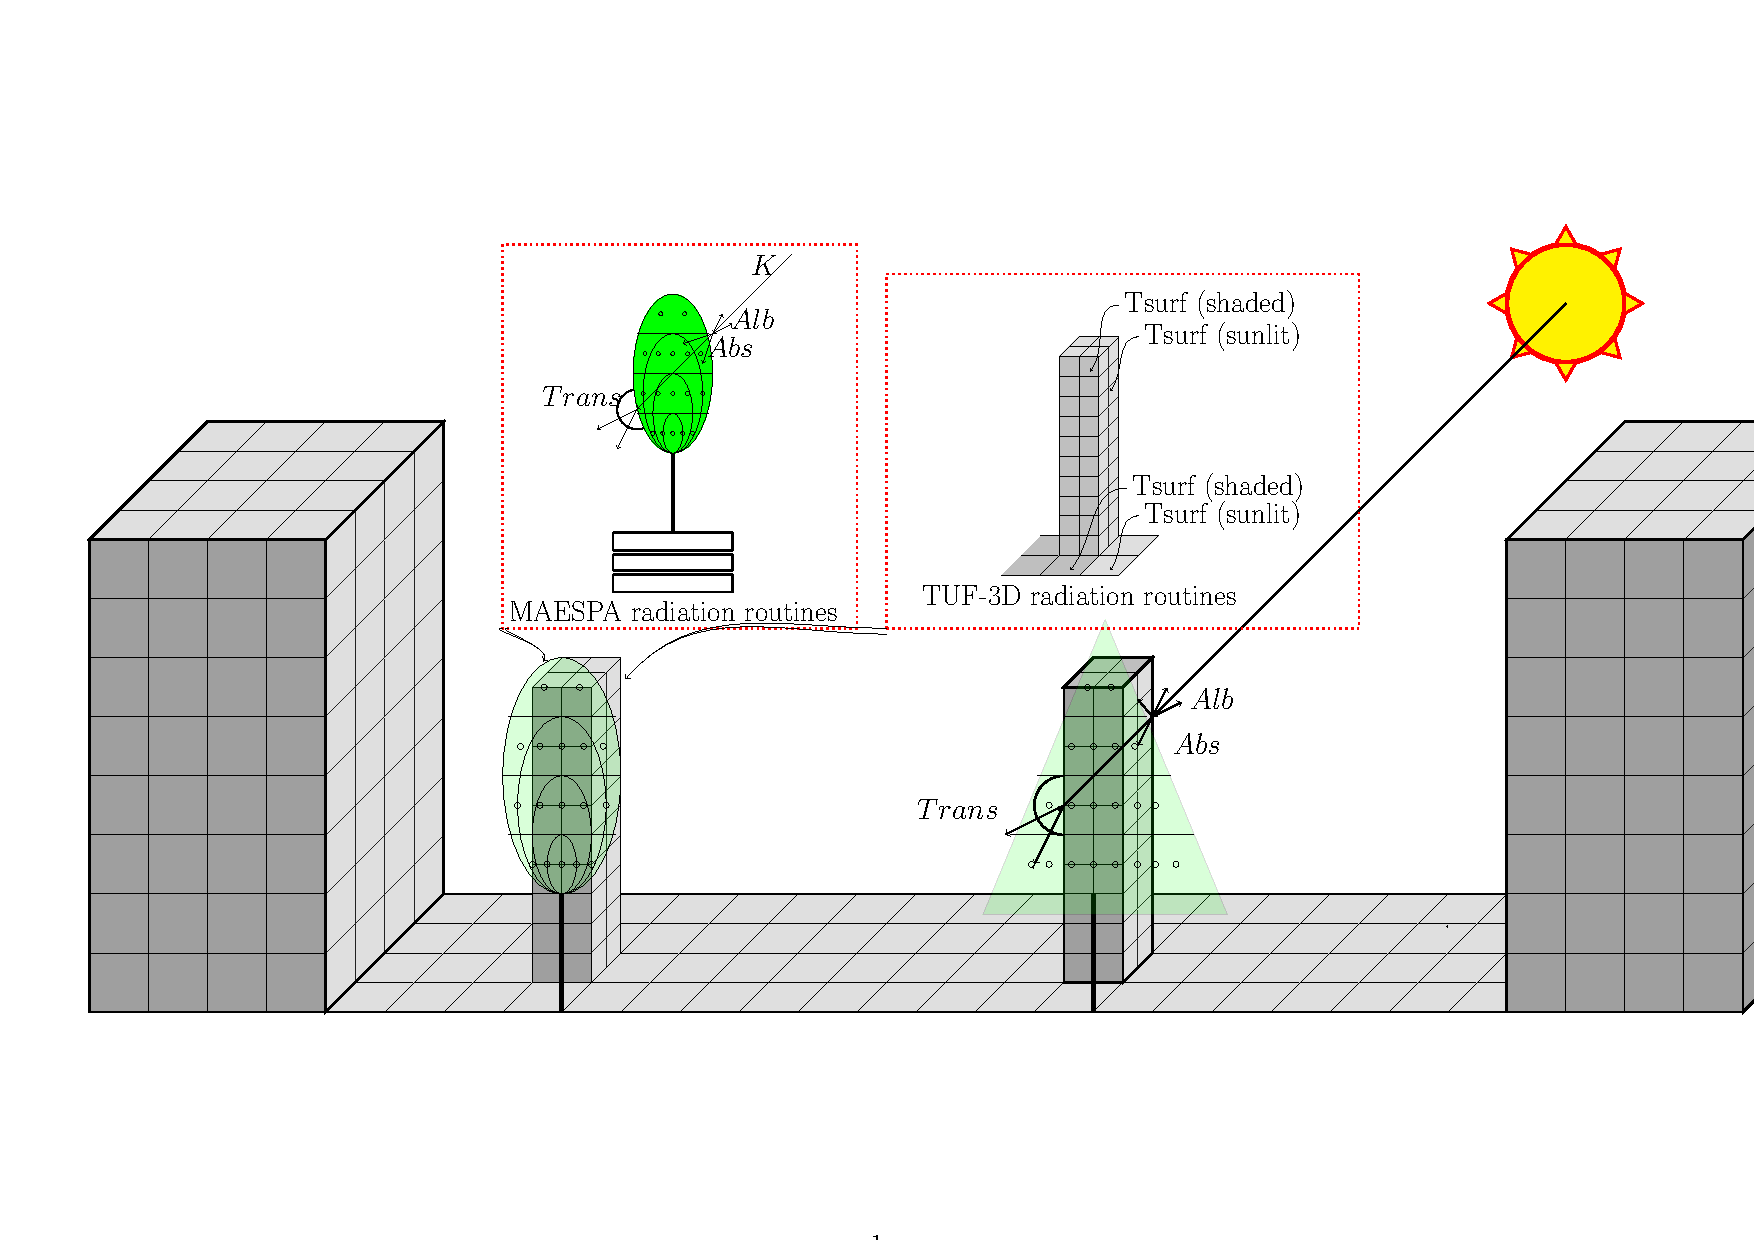
\includegraphics[trim = 15mm 41mm 0mm 31mm, clip, scale=0.45]{images/TUFWithMaespaVegRadiation.pdf}  
 \caption{Integration of MAESPA tree model into VTUF-3D radiation fluxes routines, in which tiled instances of MAESPA vegetation (in green) are used to calculate radiation transmission for VTUF-3D placeholder vegetation structures (in grey)\label{fig:TUFWithMaespaVegRadiation}.}
\end{figure}

The second major change required is including the physiological processes of vegetation and soil in the model. Using a novel approach, MAESPA tiles replace VTUF-3D ground surfaces with vegetated MAESPA surfaces and use results of MAESPA’s photosynthesis and water balance routines to modify VTUF-3D's energy balance calculations. The vegetation is treated as a flat two dimensional ground surface tile for the surface energy balances. However, each embedded MAESPA surface actually models a full 3 dimensional tree (along with associated soil and vertical movement of water) and feeds results back to VTUF-3D ground surface energy balances (Figure \ref{fig:TUFWithMaespaInsert}).

%The second major change required is including the physiological processes of vegetation and soil in the model. Using a novel approach, MAESPA tiles replace VTUF-3D ground surfaces with vegetated MAESPA surfaces and use results of MAESPA's photosynthesis and water cycle routines to modify VTUF-3D's energy balance calculations. Each embedded MAESPA surface calculates a full 3 dimensional tree (along with associated soil and movement of water) and feeds results back to VTUF-3D ground surface energy balances (Figure \ref{fig:TUFWithMaespaInsert}). 

\begin{figure}[!htbp]
 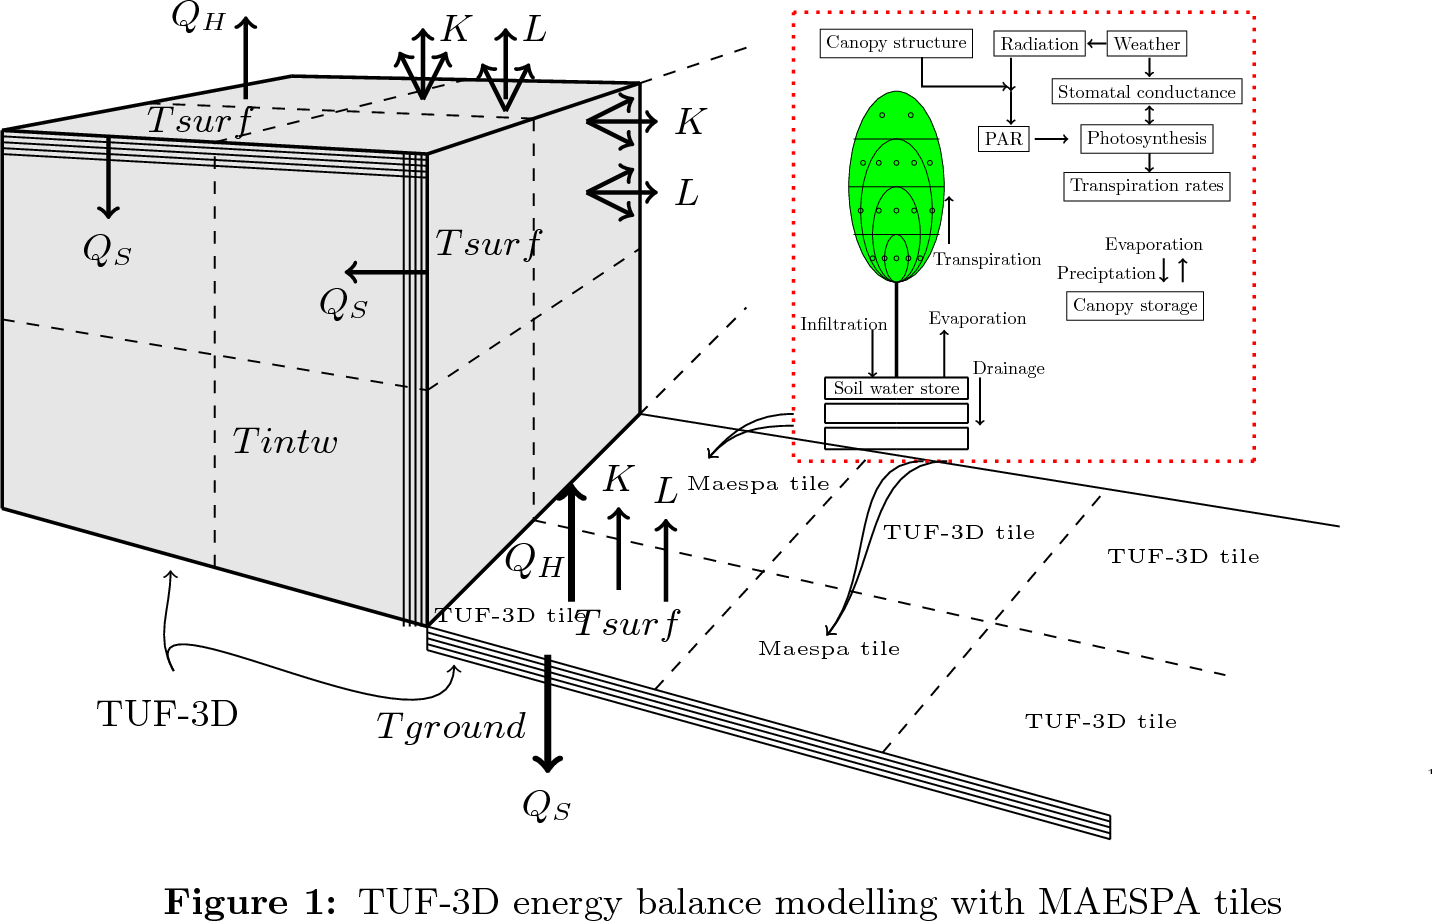
\includegraphics[trim = 0mm 14mm 22mm 0.0mm, clip, scale=0.25]{images/TUFWithMaespaInsert.png}
 \caption{\label{fig:TUFWithMaespaInsert} In VTUF-3D energy balance modelling, ground surfaces can contain either regular TUF-3D surfaces or a surface containing MAESPA modelled vegetation. All surfaces will calculate energy balances at the conclusion of each timestep, partitioning available energy into radiative and storage fluxes. Those surfaces with vegetation will also account for vegetation physiological processes when performing energy balances.}
\end{figure}

At the conclusion of each timestep (default of 30 minutes but duration is user configured), VUF-3D calculates the energy balance of each surface. Incoming radiation energy and existing stored energy are partitioned into new values of stored and radiated heat. A variable for latent energy has been added to the model and energy is allocated to it from the pool of available energy. Tiles of MAESPA instances (with an individual tree or other types of vegetation in each) are used for surfaces that have vegetation (Figure \ref{fig:TUFWithMaespaInsert}). These instances provide values of radiation transmission, energy fluxes, and soil water storage for each item of vegetation in the domain using their unique properties and characteristics. If a surface does not contain vegetation, VTUF-3D runs its normal energy balance calculations.


%\subsection{Model description}
In the following sections, the VTUF-3D model is detailed. VTUF-3D is constructed using the TUF-3D model, as described in \cite{Krayenhoff2007}, leaving all its components largely unchanged except for the two interactions as described in the overview of changes (Section \ref{sec:DesignOverview}). The vegetation functionality is added through the MAESPA model, described in \cite{Duursma2012}, with some of its components running in parallel and replacing some of the TUF-3D components in some parts of a modelled domain. The linkage components will be described later in this article in the model integration section (Section \ref{sec:integration}).

%\subsection{Radiative processes}
\subsection{Radiative transfer}\label{sec:radiativetransfer}

In order to track the movement and allocation of radiation, VTUF-3D’s modelling domain is built up in 3-D using cubes and their surfaces (facets). Ray tracing determines the visibility of each surface to each other, matched using plane parallel analytical equations of \cite{Siegel2001} and \cite{Hottel1967}. Ray tracing also determines sunlit and shaded patterns on the 3D urban surfaces throughout a simulation using a modified version of the \cite{Soux2004} algorithm. Reflections and absorption of longwave and shortwave radiation are modelled using a radiosity approach (radiative reflection and emission treated as perfectly diffuse). All the specific details of these radiative transfer calculations are contained in \cite{Krayenhoff2007}.

For vegetated parts of the domain, radiative transfer is calculated by components from MAESPA. Incoming radiation, both photosynthetic radiation (PAR) and near infrared (NIR) is partitioned into direct and diffuse using \cite{Weiss1985}. Canopy structure is calculated based on \cite{Wang1990}, supporting a variety of crown shapes namely: conical, half-ellipsoidal, ellipsoidal and paraboloidal. Absorption and scattering of radiation (PAR, NIR, and thermal radiation) by the canopy is calculated using \cite{Norman1979}. Full details of all calculations are included in \cite{Duursma2012}.

Net radiation, is calculated in Equation (\ref{eq:rnet}) ($Q^{*}_{veg}$ for vegetated grid squares, otherwise $Q^{*}$ for non-vegetated grid squares), 


\begin{equation}\label{eq:rnet}
\begin{split}
Q^{*}_{veg} =& K\downarrow - (\alpha _{veg} K\downarrow) + \epsilon _{veg} L\downarrow - \epsilon _{veg} \sigma  (T_{sfc,veg}) ^{4} 
\\
Q^{*} =& K\downarrow - (\alpha K\downarrow) + \epsilon L\downarrow - \epsilon \sigma  (T_{sfc}) ^{4} 
\end{split}
\end{equation}

where $K\downarrow$ is the downward shortwave radiative flux density (W m$^{-2}$), $L\downarrow$ is the downward longwave radiative flux density (W m$^{-2}$), $\alpha _{veg}$ of vegetation is set to 0.20 and $\epsilon _{veg}$ of vegetation set to 0.97 \citep[p. 12]{Oke1987z}, otherwise $\alpha$ and $\epsilon$ (of non-vegetated surfaces) are set to user configured values (model default values are 0.10 and 0.92 \citep{Krayenhoff2007}), and $\sigma$ is the Stefan-Boltzmann constant (=5.67 $\times$ 10$^{-8}$W m$^{-2}$K$^{-4}$), and $T_{sfc,veg}$ is the vegetation surface temperature (K), or $T_{sfc}$ for non-vegetated surfaces.

\nomenclature{$K\downarrow$}{downward shortwave radiative flux density (W m$^{-2}$)} 
\nomenclature{$L\downarrow$}{downward longwave radiative flux density (W m$^{-2}$)}
\nomenclature{$\alpha _{veg}$}{shortwave albedo of vegetation}
\nomenclature{$\epsilon _{veg}$}{longwave emissivity of vegetation}
\nomenclature{$\alpha$}{shortwave albedo }
%\nomenclature{$\sigma$}{Stefan-Boltzmann constant (=5.67 $\times$ 10$^{-8}$W m$^{-2}$K$^{-4}$)} 
\nomenclature{$T_{sfc,veg}$}{vegetation surface temperature (K)} 

\nomenclature{$T_{sfc}$}{surface temperature (K)} 
\nomenclature{$Q^{*}_{veg}$}{calculation of vegetation net radiation flux density (W m$^{-2}$)}
\nomenclature{$Q^{*}$}{net radiation flux density (W m$^{-2}$)} 

\subsection{Convective energy fluxes}

As the simulation proceeds through each timestep, an energy balance is performed on each surface. For each surface with vegetation, the surface temperature ($T_{sfc}$) is set to the value calculated by MAESPA for that tree. The following describes the differences that the unmodified TUF-3D uses to calculate the energy balances needed by VTUF-3D to partition the energy fluxes of a vegetated surface.

\subsubsection{Latent energy fluxes}
%%%\subsubsection{Calculation of leaf temperature and leaf water potential}
\label{sec:calcleaftemp}
\nomenclature{$Q_{E}$}{latent heat flux (W m$^{-2}$)}
\nomenclature{$Q_{E,veg}$}{calculation of vegetation latent heat flux (W m$^{-2}$)} 

For latent energy fluxes ($Q_{E}$), $Q_{E,veg}$ is the value for the grid square calculated in the MAESPA tree calculations, loaded from the MAESPA data for the individual item of vegetation and accompanying soil. Physiological processes and the water balance are modelled by MAESPA supporting the soil-plant-atmosphere continuum. Stomatal conductance within the vegetation uses MAESPA components based on the widely used Ball-Berry type approach \citep{Ball1987,Duursma2012}. Options are available to use a number of variations including: the Ball-Berry model \citep{Ball1987}, the Ball-Berry-Leuning model \citep{Leuning1995}, the Ball-Berry-Opti model \citep{Medlyn2011}, the Tuzet model \citep{Tuzet2003}. The use of this stomatal conductance approach requires more detailed parameters than the `Big Leaf' stomatal resistance scheme \citep{Bailey1981,Kowalczyk1991} which only provides a canopy-wide average. This allows precise modelling of individual species and specimens of vegetation, accounting for variations of vegetation type, canopy size, and vegetation health \citep{Duursma2012}. Each individually modelled element of vegetation can be placed precisely in a modelling domain scenario.

TODO THIS SECTION NEEDS TO BE FIXED
 

Stomatal conductance is used for the calculation of leaf temperature. $E_{L}$, leaf level transpiration rate ($\mu$mol m$^{-2}$s$^{-1}$) is calculated to find $\Psi_{L}$, the leaf water potential ($MPa$) (i.e. solving the Tuzet variation of the Ball-Berry stomatal conductance), and to estimate leaf temperature throughout the canopy. For each grid point, $E_{L}$ is calculated with the Penman-Monteith equation, using the boundary layer conductance and total conductance (all detailed in the next section, Section \ref{sec:totalcanopy}). Leaf temperature is found by iteratively closing the energy balance of the leaf, based on \cite{Wang1998}. See \cite{Duursma2012} for complete details.

%%%\subsubsection{Total canopy transpiration}
\label{sec:totalcanopy}
TODO THIS SECTION NEEDS TO BE FIXED

Finally, canopy transpiration, for a MAESPA tile, is calculated using the Penman-Monteith equation \citep{Penman1948,Monteith1965}. It is calculated by summing the application of the equation to each grid point using the calculated amounts of absorbed radiation (PAR, NIR, and thermal) for each tree. $g_{B}$, the boundary layer conductance (mol m$^{-2}$s$^{-1}$), and $g_{V}$, the total conductance to water vapour (mol m$^{-2}$s$^{-1}$), are calculated using \cite{Jones1992}. The output of the canopy transpiration is used in Section \ref{sec:calcleaftemp} for leaf temperature calculations. See \cite{Duursma2012} for complete details.

%%%\subsection{Water balance}
\label{sec:waterbalance}
Water balance functionality is supplied by MAESPA modules. Each item of vegetation will be individually modelled using a single instance of MAESPA, supported by the built in water balance routines. Soil layers are configurable (set to 10 by default). Complete details of the following calculations (of all modules in Section \ref{sec:waterbalance}) are contained in \cite{Duursma2012}, thought a broad description is as follows. Infiltration is based on a function from the BROOK90 model \citep{Federer2003} infiltrating rain falling on the soil surface through the soil layers. Root water uptake calculates $F_{R}$, the cumulative fraction of fine roots to depth z (m). Next, treating the root system as a number of resistances in parallel, $E_{i}$, the root water uptake (canopy transpiration) out of layer i (mm) is calculated. In order to solve the equation simultaneously across multiple soil layers, calculations of $E_{i}$ are simplified using assumptions of \cite{Taylor1975}. Soil evaporation is only drawn through the top later and assumed to travel through a thin dry layer at the soil surface. It is based on models developed by \cite{Choudhury1988} and \cite{Williams2001}. Calculation of $E_{s}$, the rate of evaporation (mm), is based on the difference between vapour pressure differences in soil pore space and the air above. In the calculation of $G_{ws}$, the conductance of water vapour through the soil pore space (m s$^{-1}$), as the thickness of the layer of dry soil at the surface increases, more resistance to air evaporation is created. Calculation of $D_{eff}$, the effective diffusivity of the soil pore space (m$^{2}$s$^{-1}$), accounts for changes in diffusivity with changing soil temperatures. Finally, $e_{s}$, the partial water vapour pressure of the soil pore space (KPa), is calculated. 

In order to account for canopy interception of precipitation, the \cite{Rutter1975} rainfall interception model is used. In this, rain can either fall through the canopy to the ground or be intercepted by the canopy in a slowly draining canopy pool. For the second option, the canopy pool is filled until reaching a maximum volume, after which any additional rainfall immediately follows the first pathway to the ground. Some amount of water is also evaporated from the canopy. Drainage of soil water is solved downward, layer by layer, in which the change of $W_{i}$, the water storage of the layer i (mm), is calculated based on the soil hydraulic conductivity (m/s) in each layer. Hydraulics of the soil-to-leaf pathway, $k_{L}$, the total leaf-specific hydraulic conductance (mmol m$^{-2}$s$^{-1}$MPa$^{-1}$), is calculated using the total hydraulic resistance for all soil layers combined (MPa s m$^{2}$mol$^{-1}$) (estimated using the single root model of \cite{Gardner1960}).

Canopy transpiration and soil evaporation are combined to give total the $Q_{E}$ for a vegetated tile. Using MAESPA outputs of $canopystore$, $evapstore$, $soilevap$, $et$ (all in mm) (variables fully documented in \cite{Duursma2016}) are converted to W m$^{-2}$ in Equation (\ref{eq:mmtowm2})


\begin{equation}\label{eq:mmtowm2} 
  Q_{E,et} = et \times A _{mm} \times m_{mol,w} \times \Delta H_{vap} \times c_{w,kj} \times Time  
\end{equation} 
 
where $et$ is evapotranspiration (mm), $A _{mm}$ is the 2-dimensional tree area (mm$^{2}$), $Time$ is the time (seconds), $\Delta H_{vap}$, the enthalpy of evaporation (=42809 J mol$^{-1}$), $c_{w,kj}$, the conversion to watts (=1W/1000KJ/sec), and $m_{mol,w}$, the molar mass of water (=18.0152g mol$^{-1}$).

These values are combined to calculate $Q_{E}$ for a grid square in Equation (\ref{eq:lefromet})


\begin{equation}\label{eq:lefromet} 
\begin{aligned}
Q_{E} = Q_{E,et} + Q_{E,soil} + Q_{E,canopy} + Q_{E,evap} 
\end{aligned}
\end{equation}

where $Q_{E,et}$, the latent heat flux calculated from $et$ (W m$^{-2}$), $Q_{E,soil}$, the latent heat flux calculated from $soilstore$ (W m$^{-2}$), $Q_{E,canopy}$, the latent heat flux calculated from $canopystore$ (W m$^{-2}$), and $Q_{E,evap}$, the latent heat flux calculated from $evapstore$ (W m$^{-2}$).

%Each item of vegetation is modelled in its own MAESPA instance, so each tree must be loaded and processed separately. MAESPA outputs hourly transpiration in units of $mm$, so they must be converted to W m$^{-2}$ of latent energy to be used in the VTUF-3D flux re-partitioning. There is a conversion step required to calculate $Q_{E,et}$, the latent heat flux calculated from $et$ (W m$^{-2}$), using the 2-dimensional area of the tree and the time duration of each timestep in Equation (\ref{eq:mmtowm2})



With these additions, VTUF-3D is now able to account for the evapotranspiration influence of urban vegetation. The water cycle components supplied by MAESPA modelled vegetation supplies estimates of canopy and soil evaporation and evapotranspiration. Through scaling and conversion of these estimates to units of W m$^{-2}$, the model is able to account for $Q_{E}$ in energy balance partitioning, and thus account for this influence of water and vegetation on temperature predictions in urban canyons.


\subsubsection{Convective sensible heat fluxes and canopy layer air temperature (T$_{can}$)}\label{sec:convection} 
Convection in TUF-3D is implemented as an adaptation of the facet-averaged approach of \cite{Masson2000}. Horizontal advective exchanges are not considered, which is considered to be a reasonable approach given the well-mixed nature of canopy layer air \citep{Krayenhoff2007}. A more accurate but computationally intensive approach could be undertaken using a computational fluid dynamics (CFD) method. However, forcing by the convection between facets is likely less important than the forcing of surface temperatures through the shaded and unshaded radiation distribution and its interactions of surface material properties \citep{Krayenhoff2007}. The following convection sub-modules (of Section \ref{sec:convection}) are completely contained in TUF-3D and full details of calculations are contained in \cite{Krayenhoff2007}.

The convective sensible heat flux density (W m$^{-2}$), $H$, from a horizontal patch $i$ is calculated in Equation (\ref{eq:convh})
\begin{equation} 
H_{i} = h_{i} (T_{sfc,i}-T(z_{horz,i}))
\label{eq:convh} \end{equation} 
where $T_{sfc,i}$ is the surface temperature of patch i (K),
$h$ is the convective heat transfer coefficient (W m$^{-2}$K$^{-1}$), 
$T(z)$ is the air temperature at height z (K), and 
$z_{horz,i}$ is the height of the patch centre. Convection from walls is also calculated using Equation (\ref{eq:convh}) where $h_{i}$ is calculated in Equation (\ref{eq:convw})
\begin{equation} 
h_{i} = r_{w,i}(11.8+4.2 U_{eff}(z_{i}))-4.0
\label{eq:convw} \end{equation} 
where 
$r_{w,i}$ is the wall roughness coefficient of patch i,
$z_{i}$ is the depth to the bottom of layer i (m), and
$U_{eff}(z)$ is the effective wind speed at height z (m s$^{-1}$).


%\nomenclature{$h_{i}$}{heat transfer coefficient (W m$^{-2}$K$^{-1}$)} 
%\nomenclature{$T_{sfc,i}$}{surface temperature of patch i (K)} 
%\nomenclature{$T(z)$}{air temperature at height z (K)} 
%\nomenclature{$z_{horz,i}$}{height of patch forcing U(z) and T(z) above street level of patch i (m)} 
\nomenclature{$U(z)$}{wind speed at height z (m s$^{-1}$)}  
\nomenclature{$T_{can}$}{canopy air temperature ($z < z_{H}$) (K)} 

%\subsubsection{Wind speed profile}

The wind speed profile within the roughness sub-layer (RSL) is a log profile based on \cite{Masson2000}, \cite{Kusaka2001}, and \cite{Harman2004}. An exponential profile is used for the urban canopy, based on \cite{Masson2000} and \cite{Rotach1995}, calculating $U(z)$, the wind speed at height z (m s$^{-1}$).

%\subsubsection{Temperature profile and canopy energy budget}
\label{sec:tempprof}

The temperature profile treats canyon temperature ($T_{can}$) as constant for $z < z_{H}$ (where z$_{H}$ is the mean building height (m) of the domain and $z$ the height (m) within a domain), allowing a single canopy-air energy budget. Calculation of $T_{can}$, the canopy air temperature ($z < z_{H}$) (K), uses the energy budget of the air volume below $z = z_{H}$ in Equation (\ref{eq:tcan})

\begin{equation} 
T_{can}^{m+1} = T_{can}^{m} + \Bigg[ \frac{\Delta t(H_{can}^{m+1}-H_{top}^{m+1} )}{c_{air,H}^{m+1}}   \Bigg]
\label{eq:tcan} \end{equation} 

where m is the timestep index,
$H_{can}$ is the summed canopy patch convective sensible heat fluxes per canopy plan area (W m$^{-2}$),
$H_{top}$ is the convective sensible heat flux density between canopy air and boundary layer (W m$^{-2}$),
$c_{air,H}$ is the average heat capacity per unit plan area of air below z$_{H}$ (J m$^{-2}$K$^{-1}$), and
$\Delta t$ is the timestep size (s).

Calculation of $H_{top}$, in which 'top' is an imaginary surface at $z = z_{H}$, is performed in Equation (\ref{eq:htop})

\begin{equation} 
H_{top}^{m+1} = h_{top}^{m+1} (T_{can}^{m} - T_{a}^{m+1})
\label{eq:htop} \end{equation} 
where m is the timestep index,
$h_{top}$ is the convective heat transfer coefficient between canopy air and boundary layer (W m$^{-2}$K$^{-1}$), using \cite{Mascart1995} and $z_{0town}$, the roughness length for momentum (domain) (m), and
$T_{a}$ is the air temperature at z$_{ref}$ (K).

%\subsubsection{Stomatal conductance}\label{Stomatalconductance}



%\nomenclature{$E_{L}$}{leaf level transpiration rate ($\mu$mol m$^{-2}$s$^{-1}$)} 
%\nomenclature{$\Psi_{L}$}{leaf water potential (MPa)} 

%\nomenclature{$g_{B}$}{boundary layer conductance (mol m$^{-2}$s$^{-1}$)} 
%\nomenclature{$g_{V}$}{total conductance to water vapour (mol m$^{-2}$s$^{-1}$)} 

For sensible heat fluxes ($Q_{H}$), vegetation is accounted for differently by using the $T_{sfc}$ of the vegetation instead of the TUF-3D $T_{sfc}$ value in Equation (\ref{eq:qhveg}) and will yield a different result using the MAESPA vegetation $T_{sfc}$ than if the TUF-3D surface temperature had been used

\begin{equation}\label{eq:qhveg}
 Q_{H,veg} = h_{i}  (T_{sfc,veg}-T_{conv}) 
\end{equation}

where $h_{i}$ is a calculated heat transfer coefficient (W m$^{-2}$K$^{-1}$) (using \cite{Mascart1995} and the effective wind speed) and $T_{conv}$ is the iterative converging T$_{can}$ canyon temperature (K).

\nomenclature{$Q_{H}$}{sensible heat flux (W m$^{-2}$)} 
\nomenclature{$Q_{H,veg}$}{calculation of vegetation sensible heat flux (W m$^{-2}$)} 
\nomenclature{$h_{i}$}{heat transfer coefficient (W m$^{-2}$K$^{-1}$)} 
\nomenclature{$T_{conv}$}{converging canyon temperature (K)} 

\subsection{Conduction and surface temperatures}

Heat conduction between the layers in each surface in VTUF-3D (based on TUF-3D) is calculated in a 1-D heat conduction equation based the scheme from the Town Energy Budget (TEB) model \citep{Masson2000}. Calculating the surface temperature (the boundary condition for the surface) using the energy balance of the surface is based on a version of \cite{Arnfield1990}. See \cite{Krayenhoff2007} for complete details.


By contrast, ground storage fluxes ($Q_{G}$) of MAESPA grid squares are calculated as a residual of the energy balance equation (where $Q_{G}$ = $Q^{*}$ - $Q_{H}$ - $Q_{E}$). Calculation of $Q_{G}$ uses Equation (\ref{eq:qgvtuf}) for grid squares containing vegetation (calculating $Q_{G,veg}$), while non-vegetated grid squares calculate $Q_{G,street}$ in Equation (\ref{eq:qgtuf}) to calculate the street ground storage fluxes:

\begin{equation}\label{eq:qgvtuf}
 Q_{G,veg} =  Q^{*}_{veg} - Q_{H,veg} - Q_{E,veg}
\end{equation}

\begin{equation}\label{eq:qgtuf}
 Q_{G,street} = k_{1}  ( T_{sfc} - T_{1} ) \frac {2}{T_{m}}
\end{equation}

where $k_{1}$ is the thermal conductivity of the surface (W m$^{-1}$K$^{-1}$) , $T_{1}$ is the temperature of the shallowest layer (K), and $T_{m}$ is the temperature of the deepest layer (K).

\nomenclature{$Q_{G}$}{ground heat storage (W m$^{-2}$)}
\nomenclature{$Q_{G,veg}$}{calculation of vegetation ground heat storage (W m$^{-2}$)} 
\nomenclature{$Q_{G,street}$}{calculation of street ground heat storage (W m$^{-2}$)} 
\nomenclature{$T_{1}$}{temperature of the shallowest layer (K)} 
\nomenclature{$T_{m}$}{temperature of the deepest layer (K)} 
\nomenclature{$k_{1}$}{thermal conductivity of the surface (W m$^{-1}$K$^{-1}$)} 


%\subsubsection{Energy balance partitioning during simulation timesteps}\label{sec:parttimestep}


%\subsubsection{Surface convection}


%\nomenclature{$r_{w,i}$}{wall roughness coefficient of patch i} 
%\nomenclature{$z_{i}$}{depth to the bottom of layer i (m)} 
%\nomenclature{$U_{eff}(z)$}{effective wind speed at height z (m s$^{-1}$)} 


%%%\subsubsection{Infiltration}
%%%\subsubsection{Root water uptake}
%\nomenclature{$F_{R}$}{cumulative fraction of fine roots to depth z (m)} 
%\nomenclature{$E_{i}$}{root water uptake (canopy transpiration) out of layer i (mm)} 
%%%\subsubsection{Soil evaporation}\label{sec:soilevaporation}
%\nomenclature{$E_{s}$}{rate of evaporation (mm)} 
%\nomenclature{$G_{ws}$}{conductance of water vapour through the soil pore space (m s$^{-1}$)} 
%\nomenclature{$D_{eff}$}{effective diffusivity of the soil pore space (m$^{2}$s$^{-1}$)} 
%\nomenclature{$e_{s}$}{partial water vapour pressure of the soil pore space (KPa)} 
%%%\subsubsection{Canopy interception}
%%%\subsubsection{Drainage}
%%\nomenclature{$W_{i}$}{water storage of the layer i (mm)} 
%%%\subsubsection{Hydraulics of the soil-to-leaf pathway}
%\nomenclature{$k_{L}$}{total leaf-specific hydraulic conductance (mmol m$^{-2}$s$^{-1}$MPa$^{-1}$)} 


\subsection{Tmrt and UTCI}\label{sec:tmrtutci}

VTUF-3D provides output of incoming and outgoing shortwave and longwave radiation and $T_{sfc}$ for each facet (surface) at each time step. Air temperature for the canyon, $T_{can}$ (calculated in Section \ref{sec:tempprof}) is also provided for each timestep. Using these and values of vapour pressure from the forcing data and wind speed at street level (calculated in Section \ref{sec:convection}), the values for $T_{mrt}$ and UTCI are calculated for each surface. Options in the model are available to either calculate $L\downarrow$, using the clear sky formula of \cite{Prata1996}, or use forcing values. Based on this, different options can be used to calculate the following equations.

%\subsubsection{Globe temperature calculation}
\nomenclature{$T_{g}$}{globe temperature (K)} 
\nomenclature{$A$}{surface area of a sphere of diameter D, of value 0.15m, (=$\pi 0.15^{2}$m$^{2}$)} 
\nomenclature{$\epsilon_{a}$}{longwave emissivity of the atmosphere} 
\nomenclature{$\epsilon_{g}$}{globe emissivity (=0.95)}  
\nomenclature{$h$}{convective heat transfer coefficient (W m$^{-2}$K$^{-1}$)} 
%\nomenclature{$\sigma$}{Stefan-Boltzmann constant (=5.67 $\times$ 10$^{-8}$W m$^{-2}$K$^{-4}$)} 
\nomenclature{$T_{a}$}{dry bulb air temperature (K)} 
\nomenclature{$S$}{horizontal solar irradiance (W m$^{-2}$)}  
\nomenclature{$\theta$}{solar zenith angle} 
\nomenclature{$\alpha_{sfc}$}{surface albedo (=0.15)} 
\nomenclature{$\alpha_{g}$}{globe albedo (=0.05)} 
\nomenclature{$f_{dir}$}{fraction of the total horizontal solar irradiance, $S$, due to the direct
beam of the sun}

Calculations of mean radiant temperature $T_{mrt}$ uses a two step procedure. First, globe temperature ($T_{g}$) is calculated by an iterative relaxation solution, using a formulation of \cite{Liljegren2008} in Equation (\ref{eq:tg2}) 


\begin{equation}\label{eq:tg2}
\begin{split}
A\epsilon_{g}\sigma T_{g}^{4} &= \frac{A}{2} \epsilon_{g}\sigma( \epsilon_{a} T_{a}^{4} +  \epsilon_{sfc} T_{sfc}^{4} ) \\
&+ \frac{A}{2}( 1-\alpha_{g})(1-f_{dir})S  \\
&+ \frac{A}{4}( 1-\alpha_{g})f_{dir}S /\cos(\theta) \\
&+ \frac{A}{2}( 1-\alpha_{g})\alpha_{sfc}S \\
&- Ah(T_{g}-T_{a})   
\end{split}
\end{equation}

where $A$, is the surface area of a sphere with diameter D of value 0.15m,
$\epsilon_{a}$, the longwave emissivity of the atmosphere, 
$\epsilon_{g}$, the globe emissivity (of value 0.95), 
$h$, the convective heat transfer coefficient (W m$^{-2}$K$^{-1}$) (see Equation (\ref{eq:h})), 
$\sigma$, the Stefan-Boltzmann constant (=5.67 $\times$ 10$^{-8}$W m$^{-2}$K$^{-4}$), 
$T_{a}$, the dry bulb air temperature (K) (using $T_{can}$), 
$T_{sfc}$, the surface temperature (K), 
S, the horizontal solar irradiance (W m$^{-2}$) calculated from the total of absorbed and reflected shortwave (resulting from calculations in Section \ref{sec:radiativetransfer}), 
$\theta$, the solar zenith angle, 
$\alpha_{sfc}$, the surface albedo (of value 0.15),  
$\alpha_{g}$, the globe albedo (of value 0.05), and 
$f_{dir}$, the fraction of the total horizontal solar irradiance, $S$, due to the direct
beam of the sun. The convective heat transfer coefficient, $h$, is calculated using Equation (\ref{eq:h})

\begin{equation}\label{eq:h}
Nu = 2.0 + 0.6Re^{1/2}Pr^{1/3};  ~~h = k / D Nu
\end{equation}

where $Nu$ is the Nusselt number (-),
$Re$, the Reynolds number (-),
$Pr$, the Prandtl number (-), and 
$k$, the thermal conductivity of the fluid (i.e. air) (W m$^{-1}$K$^{-1}$) \citep{Liljegren2008}.

%\nomenclature{$Nu$}{Nusselt number (-)} 
%\nomenclature{$Re$}{Reynolds number (-)} 
%\nomenclature{$Pr$}{Prandtl number (-)} 
\nomenclature{$k$}{thermal conductivity of the fluid (i.e. air) (W m$^{-1}$ K$^{-1}$)} 

\nomenclature{$L \downarrow_{i,sky}$}{initial incident sky-derived longwave (W m$^{-2}$)} 
\nomenclature{$K\downarrow_{dif}$}{domain-level incoming diffuse shortwave (W m$^{-2}$)}
\nomenclature{$K\downarrow_{dir}$}{domain-level incoming direct shortwave (W m$^{-2}$)}
\nomenclature{$\epsilon$}{longwave emissivity}
\nomenclature{$T_{s,1}$}{soil surface temperature (K)}

Depending on user defined scenario model configuration settings, a number of terms in Equation (\ref{eq:tg2}) can use internally calculated values. $\sigma(\epsilon_{a} T_{a}^{4} + \epsilon_{sfc} T_{sfc}^{4} )$ is replaced with $L\downarrow + L\uparrow$, the result of reflections of $L \downarrow_{i,sky}$ calculated in Section \ref{sec:radiativetransfer}). $(1-f_{dir})S$ will be replaced with $K \downarrow_{dif}$ and $f_{dir}S/ \cos(\theta)$ with $K \downarrow_{dir}$. Also, for vegetated grid squares, the terms for $L\downarrow$ and $L\uparrow$ will be replaced with calculations of $L\downarrow$ and $L\uparrow$ from $\epsilon \sigma T^{4}$ where $T_{s,1}$, soil surface temperature (K), is used as the temperature term for the $L\uparrow$ calculation while leaf temperature (from Section \ref{sec:calcleaftemp}) is used for $L\downarrow$. Otherwise, the following sequence of equations are used to calculate the terms for Equation (\ref{eq:tg2}).


%\subsubsection{$T_{mrt}$ calculation}

Using $T_{g}$, calculated in Equation (\ref{eq:tg2}), the second step in calculating $T_{mrt}$ proceeds in Equation (\ref{eq:tmrtbucket}) of \cite{Kantor2011}
\begin{equation}\label{eq:tmrtbucket}
  T_{mrt} = 
  \bigg(
   (T_{g}+273.15)^{4} + 
    \frac{1.1 \times 10^{8}  ws_{cm}^{0.6}}{\epsilon_{g}  D^{0.4}}
    \times 
     (T_{g}-T_{a})
    \bigg)^{0.25} - 273.15
\end{equation}
 where $ws_{cm}$ is the wind speed (cm s$^{-1}$).

%\nomenclature{$ws_{cm}$}{wind speed (cm s$^{-1}$)} 

%\subsubsection{UTCI calculation}
Finally, the UTCI for each surface is calculated, using the \cite{Brode2009u} UTCI formula, in Equation (\ref{eq:utci})

\begin{equation}\label{eq:utci}
  UTCI = f(T_{a}, ws, rh, T_{mrt})
\end{equation}
\nomenclature{$ws$}{wind speed (m s$^{-1}$)} 

generating a UTCI value for each surface, using input of $T_{a}$, air temperature (using $T_{can}$), $ws$, wind speed (m s$^{-1}$) (using model calculated $U_{road}$, the wind speed at road level), $rh$, relative humidity (\%) (from forcing data), and $T_{mrt}$. VTUF-3D does not currently calculate a canopy level $rh$. This is a current limitation and a future enhancement for the model. This UTCI formula was designed to provide human thermal comfort assessments using thermal environment parameters with fixed values (incorporated into the formula) for metabolic rates and clothing levels \citep{Brode2012a}. While future development is needed to provide wider flexibility to vary metabolic rates and clothing levels, existing versions of this formula were developed to embody equivalent human physiological responses to differing thermal parameters \citep{Havenith2012,Fiala2012}.



\subsection{New VTUF-3D shading logic integrating vegetation shading}\label{sec:integration}
%\subsubsection{TUF-3D shading logic}\label{sec:existingshading}
In order to understand the changes made to create VTUF-3D, an overview of the TUF-3D logic is necessary. Two dimensional (x,y) locations of building locations are configured along with their heights. TUF-3D uses forcing data of temperature, humidity, incoming radiation levels, and wind speed and direction from a location at specified z height (above the canopy). Wind is used in roughness calculations but not used to resolve movements around the buildings (as a CFD based model would). This simplification is a design decision trade-off to reduce the complexity of the model and the intensity of computations, while still producing robust enough results (see Section \ref{sec:convection}).



\begin{figure}[!htbp]
%\fbox{
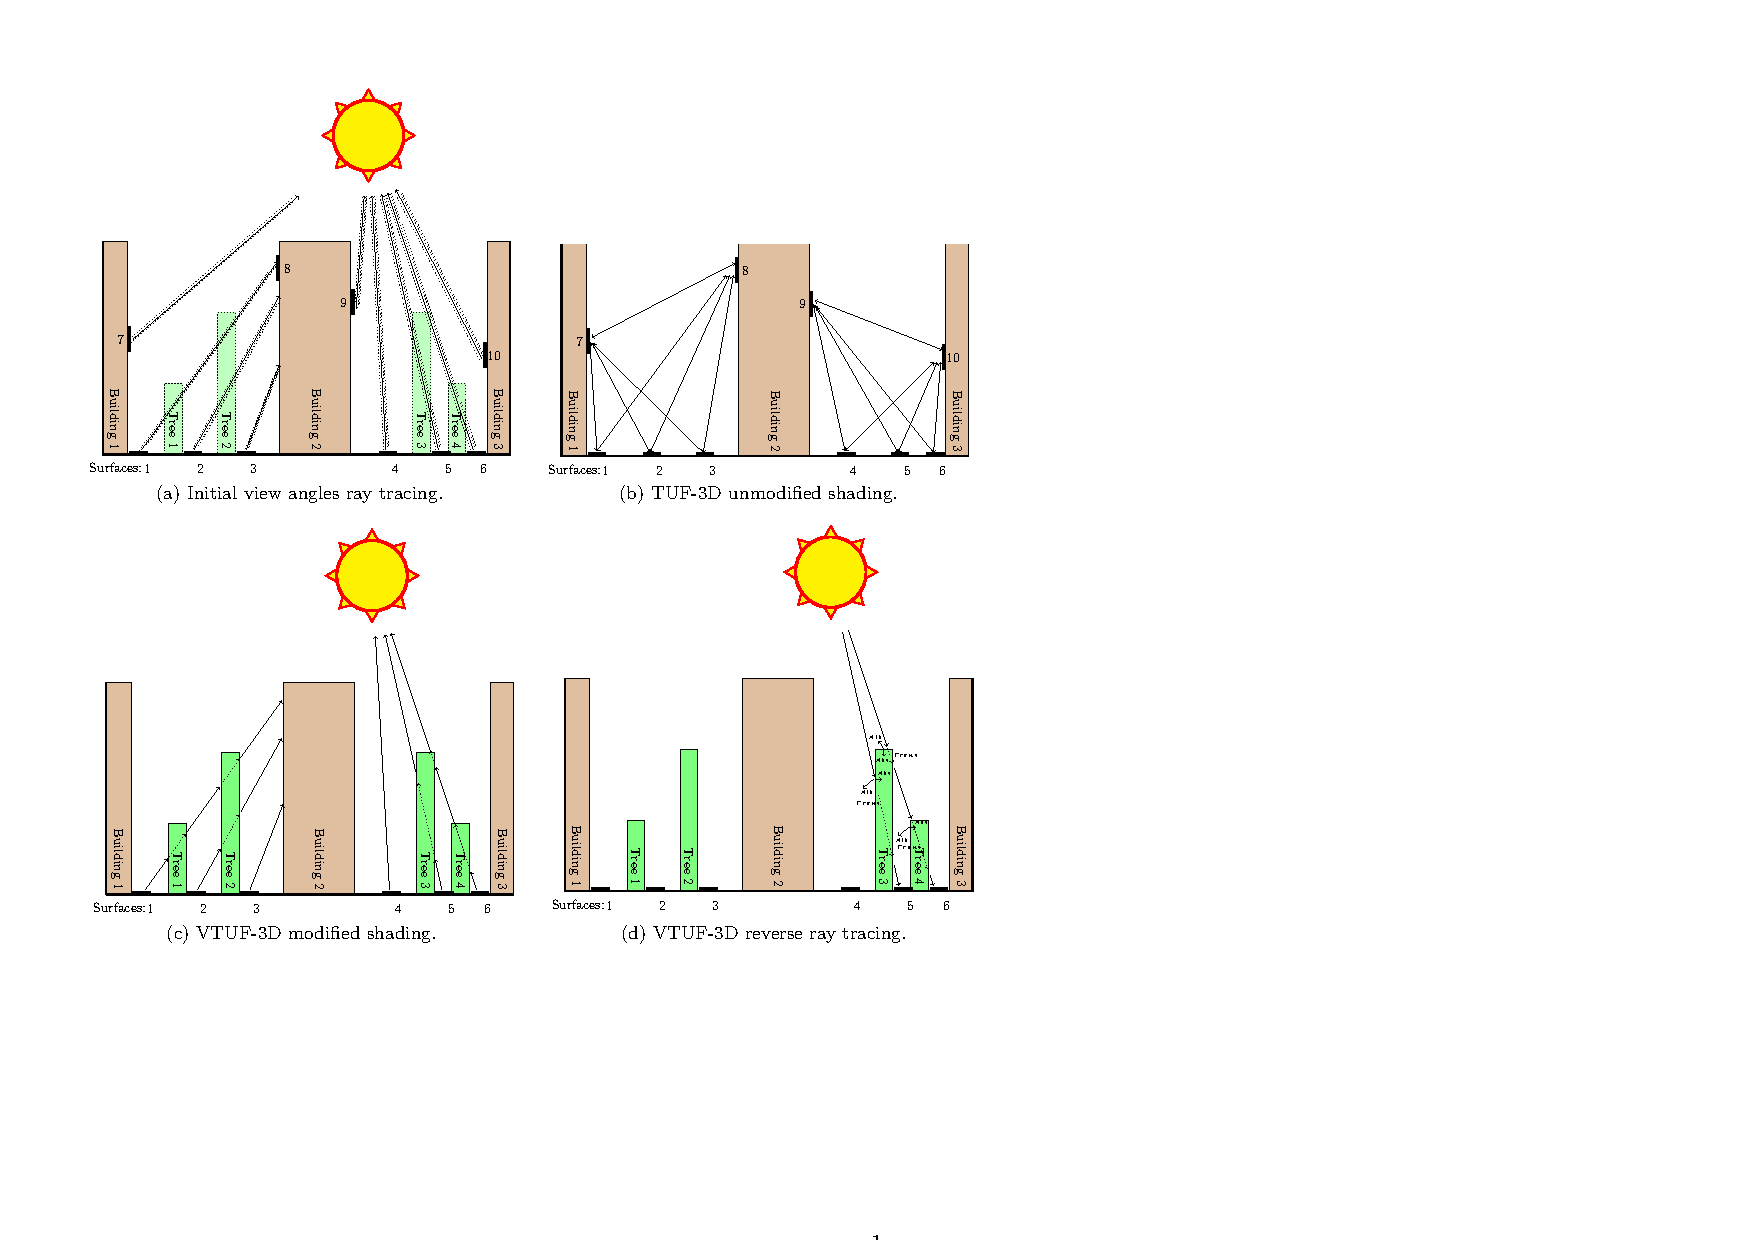
\includegraphics[trim = 15mm 50mm 132mm 15mm, clip, scale=0.75]{images/ModelDiagramsCombined2.pdf}
%   }
   \caption{(a) Initial view angles ray tracing, run during model initialisation to determine which surfaces are visible to each other. Trees depicted with dashed borders to emphasise they are present in the domain but are not considered at this point in the simulation. \label{fig:initray} (b) TUF-3D unmodified shading logic in which each surface performs four ray traces (from each surface quarter) towards the sun and determines sunlit percentage based on how many rays leave the domain without meeting an obstruction. Vegetation modelling is not possible in TUF-3D, so is not depicted. \label{fig:shading} (c) VTUF-3D modified shading, timestep ray tracing, using the same process as the unmodified logic but setting a flag for any ray that encounters vegetation. \label{fig:modshading} (d) VTUF-3D modified shading, reverse ray tracing. For any rays that encounter vegetation in forward ray tracing, reverse ray traces are performed to allocate radiation to intervening encountered surfaces. \label{fig:modshadingreverse}} 
\end{figure}

%\nomenclature{$z_{H}$}{mean building height (m)} 

During the model initialisation stage, ray tracing is done (Figure \ref{fig:initray}a) between all surfaces to determine which surfaces are visible to each other. This step reduces the number of radiative interactions of surfaces that will need to be considered throughout the simulation run. As the model runs a simulation, at each time step, TUF-3D runs a shading routine (Figure \ref{fig:shading}b). In it, the model iterates through each surface in the domain (roads and building walls and roofs) and ray-traces towards the sun. Each of these surfaces (patches) are divided into quarters and each of these are ray-traced from the centre of each quarter. 


Each surface keeps track of the level of illumination, the shade coefficient for that surface, at each timestep. If the ray passes to the top of the domain without being obstructed (i.e. surface 4) then 0.25 is added to the shade coefficient for that surface. If the ray is obstructed before reaching the top of the domain (i.e. surface 3), then nothing is added. Each surface has potential values of 0, 0.25, 0.5, 0.75 and 1.0. During the later energy balance step, an appropriate amount of incoming radiation is allocated to this surface based on this coefficient.

\subsubsection{Integrating vegetation shading and modified ray tracing logic in VTUF-3D}\label{sec:Representationofvegetation}

After model improvements to VTUF-3D were made, a similar parallel logic was used to represent the vegetation in the domain. These vegetation elements are ignored in the initialising ray-tracing (Figure \ref{fig:initray}a). This initial ray tracing is performed to optimise the modelling, to exclude any two surfaces which will never be visible to each other. However, depending on the density of the vegetation, a particular ray trace might not be completely obscured by vegetation so these cases will have to be evaluated during the simulation run.

At each time step during the simulation, VTUF-3D now runs a modified shading routine (Figure \ref{fig:modshading}c). During the model iteration through each surface in the domain, ray-traces towards the sun are done as described previously. However, each step of the ray trace checks to see if vegetation has been encountered. If vegetation is encountered, a vegetation encountered flag is set. Then the ray trace continues and concludes when it either passes out of the domain or is blocked by a building. 

To resolve the sunlit factor for surfaces that encountered vegetation during the ray trace, reverse ray tracing is done for those beams (Figure \ref{fig:modshadingreverse}d). For surfaces 5 and 6 in Figure \ref{fig:modshadingreverse}d, ray tracing is done from the top of the domain back along the radiation path. When the ray encounters vegetation (surfaces 5 and 6), VTUF-3D looks up the tree associated with the ground surface below and loads the offline calculations of the amount of radiation reflected, absorbed, and transmitted through the vegetation. The ray tracing continues, allocating the remaining radiation either to further intercepting vegetation or ultimately to the ground surface. Through this reverse ray tracing process, the problem of zero to many surface interceptions is solved by allocating radiation as it is transmitted from the sun and transmits through the zero to many objects it encounters along its path. 

%\subsubsection{MAESPA vegetation transmission and energy balance functionality overview}\label{sec:MAETrans}

%MAESPA, as originally designed, allows modelling of a stand of trees or of a single grid square containing a single tree. VTUF-3D uses this functionality from MAESPA in two different ways. The first is MAESPA's calculations of radiation movement through the vegetation canopy. Each tree in the VTUF-3D modelling domain is individually modelled by MAESPA before the main modelling run and then these data are extracted by VTUF-3D and used throughout the simulation. 
%
%
%Through these shading modifications, VTUF-3D stores states of and represents vegetation through placeholder simple block structures in VTUF-3D (Figure \ref{fig:TUFWithMaespaVegRadiation}), but calculates the underlying processes using their true shapes and types through the MAESPA representation. Calculated transmission values are used to distribute radiation to the appropriate surfaces during the reverse ray tracing process to determine how much radiation is scattered by the vegetation, radiation absorbed by the vegetation, while the remaining amount of radiation is then distributed to subsequent vegetation, and ultimately to the ground surface at the end of the ray. 
%
%The second integration of MAESPA is used in the surface energy balances. Flux amounts (pre-calculated offline) for each vegetation element for each time step are loaded at the beginning of the simulation and used to repartition the energy fluxes for those surfaces with vegetation on them, using the appropriate values for either sunlit or shaded vegetation. 


%\subsubsection{VTUF-3D use of MAESPA differential shading values}\label{sec:4diffshading}

In order to account for inter-tree shading or shading by buildings, each tree in the domain is modelled twice, using varied amounts of incoming shortwave. The first uses 100\% total incoming solar radiation for when the tree is fully exposed. The second uses only the diffuse component of incoming solar radiation values only for trees when shaded by obstructions. Forcing data needs to be provided by the user (as well as flagging the diffuse variation values as 0\% direct beam so MAESPA will not attempt to partition the amounts into direct/diffuse) and the proper data variation for each tree is chosen during the model run. As shortwave radiation levels vary in locations in an urban canyon across the diurnal cycle, the use of these differential values captures the differing vegetation responses. This includes varying levels of photosynthesis due to lower levels of PAR, changes in surface temperatures, and varying vegetation evapotranspiration due to differences in stomatal conductance and vapour pressure deficits.

\section{Model set up and validation}
\subsection{Model validation}







%The VTUF-3D v1.0 model has been validated using an extensive validation process to ensure that a number of different aspects of the model are functioning properly and is suitable for the task of assessing WSUD impacts on HTC. The validation used three different observational datasets. A validation against flux tower observations \citep{Coutts2007}, is detailed in the next section and VTUF-3D is found to show good performance in partitioning fluxes. In addition, it will be shown that VTUF-3D's performance is above the mean and close to maximum performance of other urban models, as analysied by \cite{Best2012}. 
%
%Two additional validations were performed and will be discussed in a forthcoming paper. In these, a validation showed VTUF-3D's ability to accurately model spatial and temporal patterns of $T_{mrt}$ and $UTCI$ across two differing urban canyons, using observations from George St. and Gipps St. in the City of Melbourne \citep{Coutts2015,White2012}. Finally, a last validation tested VTUF-3D's ability to reproduce the temporal patterns of vegetation physiological responses seen in the observations of street tree transpiration due to urban canyon geometry effects. These observations were based on a  tree study campaign recorded at Smith St. in Melbourne \citep{Gebert2012,Coutts2014a} and it was demonstrated that VTUF-3D was able to successfully capture these patterns.

%\subsection{Model validation using Preston flux observations}\label{sec:PrestonValidations}
\nomenclature{$Q_{F}$}{anthropogenic heat (W m$^{-2}$)}

Validations of VTUF-3D need to be performed to ensure that this new model is making accurate predictions. As an energy balance model, modelled output comparisons to observations of energy fluxes and temperatures are considered fundamental validations \citep{Masson2002a}. With the addition of vegetation modelling, it is important that those aspects are also properly validated. To validate VTUF-3D's accuracy in partitioning fluxes, a validation was performed based on flux tower observations recorded in the suburb of Preston, in northern Melbourne, Australia \citep{Coutts2007}. Preston is a homogeneous, low to medium density area and characterised as LCZ6B \citep{Stewart2012b}. A 40 meter flux tower recorded observations during 2003 and 2004 \citep{Coutts2007}, providing observed values of $Q^{*}$, $Q_{H}$, $Q_{E}$, air temperature, humidity, wind speed and direction. $Q_{G}$ was calculated as a residual of the surface energy balance. Estimates of the anthropogenic heat flux ($Q_{F}$) were made using an inventory approach, though $Q_{F}$ is included implicitly in the observations and contributes to the observed sensible heat fluxes. The use of this data set allows validation of surface energy balances against modelled predictions. This data set was also used as the forcing and comparison data set for Phase 2 and 4 of the International Urban Energy Balance Models Comparison Project \citep{Grimmond2011,Best2012}. Phase 2 of this comparison project evaluated the performance of 32 urban land surface modelling schemes, forced by and comparing to these observations, using a consistent methodology. Phase 4 re-evaluated many of these modelling schemes for their performance across a variety of seasonal cycles.

\subsection{Model set up}

A modelled domain (100x100m with a 5m grid resolution) was an area of interest (AOI), chosen to be representative of the overall land cover influencing the fluxes at the tower (Figure \ref{fig:PrestonModArea}). Aerial imagery from 2015 \citep{GooglePreston2015} was used as an initial basis for the modelling domain. The measurement height for the observations ensured that the measured fluxes well represented the local scale (10 to 1000 meters) of the area \citep{Coutts2007}. Additionally, the site selection ensured a homogeneous nature of the overall flux coverage area \citep{Schmid1994}. Because of this, the micro-scale modelled domain is representative of the observed fluxes observed at a local scale. This is confirmed by the land surface classification of the site. \cite{Coutts2007} undertook a land surface classifications to support interpretation of the 2003-04 flux data, from aerial imagery (from 2002) within a 500 m radius of the observation tower. The selected AOI (Figure \ref{fig:PrestonModArea}) is in good agreement with the 500 m radius classification of \cite{Coutts2007} with respect to the pervious/impervious fractions. Breakdowns of both classifications, and the 100m x 100m domain used here are shown in Table \ref{tab:expertValues}. Overall, the modelled domain selection is very similar to the broader area, is representative of the local scale and will allow an appropriate comparison between the observed and modelled results. In addition to the land cover fractions, other properties of the observation site are listed in Table \ref{tab:prvalpara}.

\begin{figure}[!htbp]
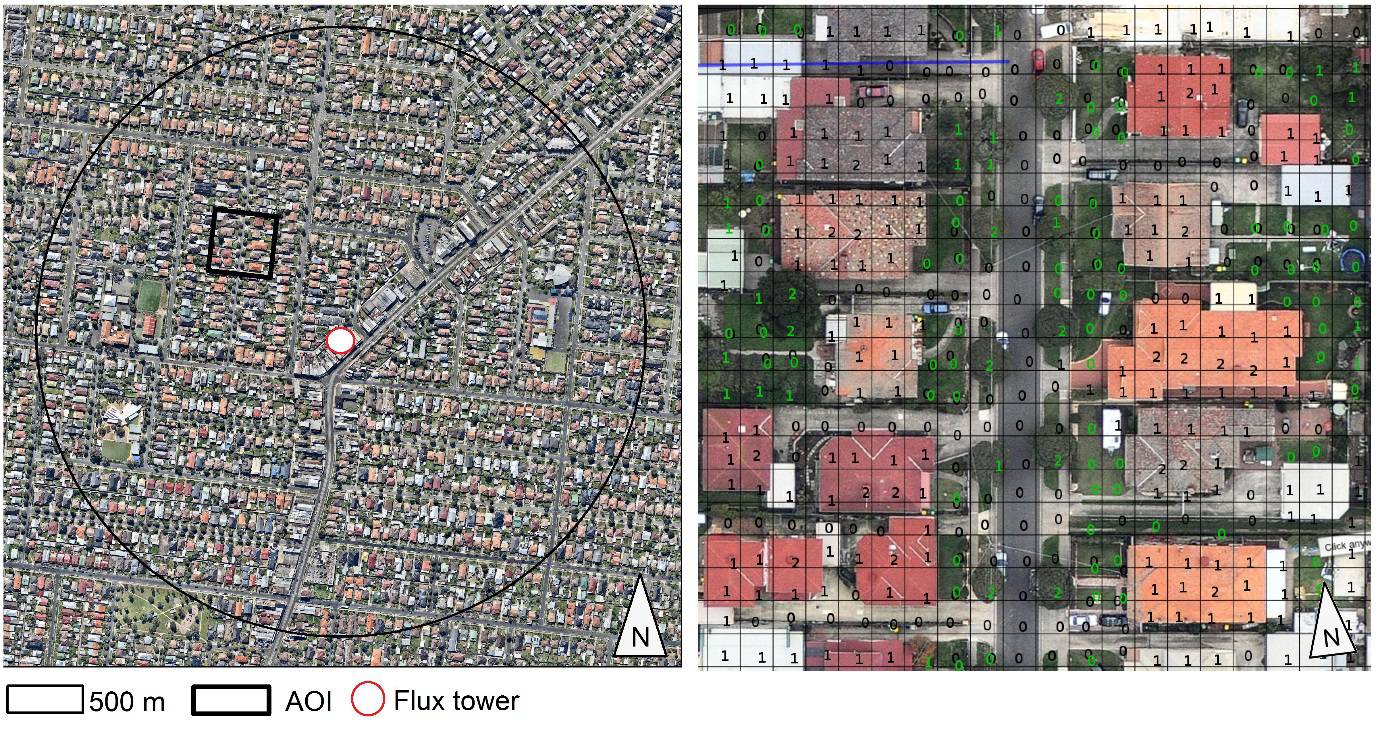
\includegraphics[trim = 0mm 0mm 0mm 0mm, clip, scale=1.00]{images/PrestonModelledArea.png} 
\caption{Observed Preston suburb showing 500m effective radius of flux tower observations. Black box annotates model domain area of interest (AOI). Adapted from \cite{GooglePreston2015}.\label{fig:PrestonModArea} / Digitisation of AOI, Preston suburban street, Oakhill Ave. Building heights in black, vegetation heights in green (in 5m units). Adapted from \cite{Nearmap2015}.\label{fig:PrestonDigitization}}      
\end{figure}

\begin{table}[!htbp]
\caption
{Preston land cover classification of a 500m radius from the observation tower from \cite{Coutts2007} and \cite{Nury2015}, and the classification of the model domain area of interest (AOI) (all in percentages). \label{tab:expertValues}} 
\begin{tabular}{ |c |c| c | c |c |c |c|p{1.65cm}|p{1.65cm}| } 
\hline \textbf{Source} & \textbf{Blg.}&	\textbf{Imp.}&\textbf{Tree}&\textbf{Grass}	&\textbf{Water}&\textbf{Tot. Imp.}&\textbf{Tot. Per.} \\ \hline
\textbf{500m radius} & & & & & &	&  \\ \hline 
\cite{Coutts2007} &44.5 &17.5&22.5 &15.0 &0.5 &62.0 &38.0	  \\ \hline 
\cite{Nury2015} &32.0 &34.5 &10.1 &23.4 &0 &66.5 &33.5  \\ \hline 
 & & & & & &	&  \\ \hline 
AOI (100x100m) &45.2 &19.3 &16.0 &19.5 &0 &64.5	&35.5  \\ \hline 
\end{tabular} 
\end{table}  
 
\begin{table}[!htbp]
\caption{Preston validation site properties \citep{Coutts2007}. \label{tab:prvalpara}}     
\begin{tabular}{| l | l |}
\hline
\textbf{Property} & \textbf{Value(s)} \\ \hline
$\alpha$, albedo & 0.15  \\ \hline
$z_{m}$, instrument height (m)&  40  \\ \hline
$z_{0}$, roughness length (m)& 0.4  \\ \hline
$z_{h}$, maximum height of roughness elements (m)& 12  \\ \hline
$z_{b}$, mean building height (m)& 6.4  \\ \hline
$H:W$, mean height to width ratio& 0.42  \\ \hline
$W:P$, mean wall-to-plan ratio &0.4  \\ \hline
\end{tabular}
\end{table}

The 2015 imagery used here for the model domain was 13 years after the 2002 imagery used in \cite{Coutts2007}. An analysis by \cite{Nury2015} of the Darebin Council area (55.6 km$^{2}$) (which includes Preston) was available, developed using aerial imagery from 2009 and LIDAR data from 2008. This was compared because the land surface classification was much improved in terms of accuracy (due to higher quality and higher resolution imagery) than that of \cite{Coutts2007} and provided a more recent set of land surface data (Table \ref{tab:expertValues}). Some differences in the classification were seen, with the Nury (2015) classification showing a lower building fraction and a higher impervious surfaces. Further, some reduction in vegetation cover is seen between the \cite{Coutts2007} classification and the \cite{Nury2015} classification. This introduces a small amount of uncertainly in the exact make-up of the modelling domain and could explain some of the low predictions of Q$_{E}$ seen later in this validation. While this dataset is at a different scale and from a later time period, it does show good agreement with the total impervious/pervious fraction of the 500m classification.


Model parameters were set to the values given in Table \ref{tab:modprvalpara} and domain parameter values in Table \ref{tab:expertValues}. Most of these values are TUF-3D default values, from \cite{Krayenhoff2007}. The modelled domain is a digitisation of the AOI, Oakhill Ave. in Preston (Figure \ref{fig:PrestonModArea}) with building locations and heights as shown in Figure \ref{fig:PrestonBldHt}.


\begin{table}[!htbp]
\caption{Preston validation scenario model parameters. \label{tab:modprvalpara}}     
\begin{tabular}{| p{8.0cm} | l | l|}
\hline
\textbf{Parameter} & \textbf{Value(s)} & \textbf{Source}\\ \hline
Albedo (roof, street, wall)   & 0.15, 0.10, 0.30   & \cite{Krayenhoff2007}\\ \hline
Emissivity (roof, street, wall)   & 0.92, 0.92, 0.88   & \cite{Krayenhoff2007}\\ \hline
Forcing data height (m)  & 40   & \cite{Coutts2007} \\ \hline
Mean height of buildings (m)  & 5.61   & Calculated from domain \\ \hline
Mean height of trees (m)  & 5.7   & Calculated from domain \\ \hline
Initial $T_{sfc}$ (roof, street, wall) (\SI{}{\degreeCelsius})  & 18.0, 23.0, 22.0  & \cite{Krayenhoff2007}  \\ \hline
Constant building internal air temperature (base of roofs and walls) (\SI{}{\degreeCelsius})  & 22.0, 20.0 & \cite{Krayenhoff2007}   \\ \hline
Constant deep-ground temperature (\SI{}{\degreeCelsius})  & 19.0  & \cite{Krayenhoff2007} \\ \hline
Constant building internal floor temperature (\SI{}{\degreeCelsius})  & 15.0  & \cite{Krayenhoff2007} \\ \hline
\end{tabular}
\end{table}

\begin{figure}[!htbp]
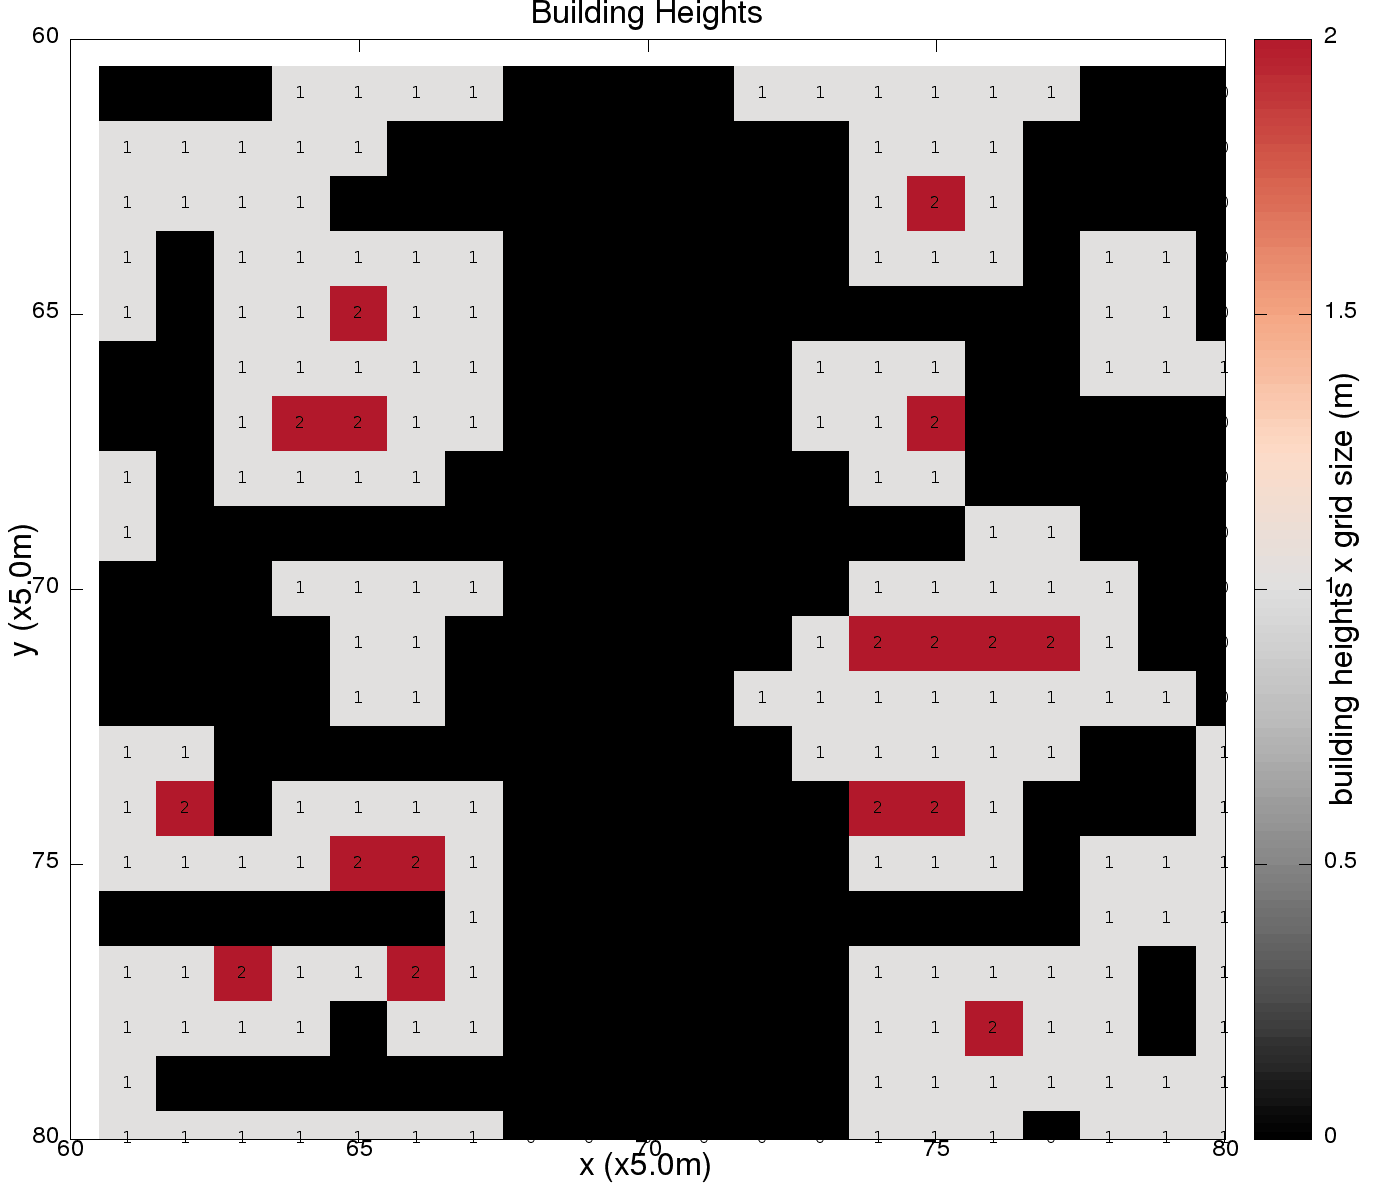
\includegraphics[trim = 0mm 0mm 0mm 0mm, clip, scale=0.20]{images/CentralBuildingHeights.png} 
\caption{Preston validation domain configured building heights (0, 5, 10m) and locations for modelling scenario Pr04Val.\label{fig:PrestonBldHt}}      
\end{figure}

%\begin{figure}[!htbp]
%\includegraphics[trim = 0mm 0mm 00mm 0mm, clip, scale=0.80,width=\textwidth]{/home/kerryn/git/Images/PrestonOverall1.png}
%\caption{Preston suburb and modelled area. Adapted from \cite{GooglePreston2015}.\label{fig:PrestonModArea}} 
%\end{figure}

%\cite{Coutts2007} provides expert and manual classifications (done at the time of the observations, 2003-2004) from aerial imagery (from 2002) within a 500m radius of the observation tower. The selected modelling area is in good agreement with the 500m classification of \cite{Coutts2007} with respect to the pervious/impervious fractions. An analysis by \cite{Nury2015} of the Darebin Council area (55.6 km$^{2}$) (which includes Preston) using LIDAR data from 2008 is also included because it provides a more recent set of land surface data for the 500m radius area. Breakdowns of both classifications are shown in Table \ref{tab:expertValues}.
%
%Some reduction in vegetation cover is seen between the 2004 observation site classification and the 2008 Darebin Council area classification. This introduces a small amount of uncertainly in the exact make-up of the modelling domain and could explain some of the low predictions of $Q_{E}$ seen later in this validation. While this dataset is at a different scale and from a later time period, it does show good agreement with the total impervious/pervious fraction of the 500m classification. Overall, the modelled domain selection is very similar to the broader area, is representative of the local scale and will allow an appropriate comparison between the observed and modelled results. 

%\begin{figure}[!htbp]
%\includegraphics[trim = 0mm 0mm 0mm 0mm, clip, scale=0.30]{/home/kerryn/Documents/Work/PrestonData/Preston-5m_Heights.png}     
%\caption[Digitisation of modelled Preston suburban street]{Digitisation of Preston suburban street, Oakhill Ave. (\textbf{1}=building heights, \textbf{\textcolor{green}{1}}=vegetation heights (in 5m units)). Adapted from \cite{Nearmap2015}.\label{fig:PrestonDigitization} }     
%\end{figure}    



% Other properties of the observation site are listed in Table \ref{tab:prvalpara}.

%The modelled land cover fractions of vegetation consist of 19.5\% grass and 16.0\% trees, matching closely to published land cover classification values for data set. Modelled building densities (Figure \ref{fig:PrestonBldHt}), consisting of 45.2\% buildings and 19.3\% impervious surfaces, also match closely to published land cover classification data set values. All values are summarised in Table \ref{tab:expertValues}.



%\subsubsection{MAESPA configurations creation} \label{section:MaespaTreeConfig}


As all the vegetation parameterisations in VTUF-3D are pluggable, individual elements are added to a domain using a specific set of configuration files with many of the physical properties scaled from a base template.  Including additional vegetation types (trees, shrubs, and ground cover) into VTUF-3D can be added by populating templates with parameter values based on observations or literature values. Two tree types were employed here, namely \textit{Olea europaea} (Olive) and \textit{Lophostemon Confertus} (Queensland brushbox), as well as turf grass, tall fescue \textit{Festuca arundinacea} (tall fescue). The detailed parameterisations for these vegetation types are shown in \ref{sec:maespavegpara}. A mix of 25\%/75\% \textit{Olea europaea} and \textit{Lophostemon Confertus}) trees were used in the model. Identifying and parametrising every tree species in the domain can be time consuming, so our parametrisations were limited here to these species. The species mix was chosen to best account for density of canopy cover in the aerial imagery but given this limitation, will not completely reflect the observed species mix and might create some modelling errors from the observed fluxes. However, the two available species are representative of commonly planted trees in Melbourne. A street tree inventory by \cite{Frank2006} finds that brushbox, a native evergreen, is the most common street tree, representing 6.9\% of street trees in Melbourne. Olive trees are considered suitable for Melbourne's climate conditions (drought tolerant evergreen) and a recommended species for council street tree planting \citep{PortPhillip2010}.



 %Vegetation settings for the two tree types (a 25\%/75\% mix of olive (\textit{Olea europaea}) and brushbox (\textit{Lophostemon Confertus}) trees) as well as grass were set to the values given in the model design vegetation parametrisation section (Appendix \ref{sec:maespavegpara}). A current limitation of the model is that the available vegetation parametrisations are limited to these three vegetation types. 




The validation simulation (which is named Pr04Val) was run for 30 days, from 10 February 2004 to 10 March 2004, forced by the observations, from \cite{Coutts2007} for those days. Meteorological forcing included $K\downarrow$, $L\downarrow$, air temperature, wind speed, wind direction, and air pressure at a height of 40m. Forcing data for the vegetation components use shortwave values of mean global and mean diffuse observations taken from one minute solar observations (station 086282, Melbourne Airport) \citep{BOM2016}. For full radiation vegetation runs, the mean global irradiance was used while for diffuse runs, the mean diffuse irradiance was used. In addition, the MAESPA FBEAM variable (fraction of incident PAR which is direct-beam) is set to 0.0 in the forcing data for diffuse runs.

The validation period contained a range of conditions. The period especially features a number of hot days (over \SI{30}{\degreeCelsius}). As one of the major applications of VTUF-3D will be examining high temperature moderation of increasing tree cover, validation over a period containing these hot days is important. The observation period also contains a number of days with precipitation. In the current VTUF-3D design, precipitation will only be received in grid squares which contain vegetation and pervious surfaces. The expected impact of this is that predictions of $Q_{E}$ will be understated for days which contain precipitation. Accounting for rainfall on impervious surfaces is a current limitation of VTUF-3D (to be addressed in later versions of VTUF-3D) and caution should be used in modelling periods which contain significant rainfall. In the intended primary use of VTUF-3D, which focuses on temperature moderation in the hottest periods of the year (which contain little rainfall), this should be less of an issue. Also, in most urban areas, precipitation on impervious surfaces will be rapidly removed as stormwater.

%\begin{figure}[!htbp]a)
%{\includegraphics[width=7cm]{/home/kerryn/Documents/Work/Data/PrestonData/PrestonTempFeb2004} }
%~b)
%{\includegraphics[width=7cm]{/home/kerryn/Documents/Work/Data/PrestonData/PrestonPPTFeb2004} }
%    \caption{Preston observations during the validation period of 9 February - 10 March 2004. a) Daily temperature ranges. b) Daily precipitation. \label{fig:Prestontemprain}}    
%\end{figure}





\subsection{Validation approach}\label{sec:prvalresults}

During this validation, a number of different scenarios (described in Table \ref{tab:simscompared}) are considered and compared. The validation scenario (named Pr04Val) compares the modelled results for the 30 day run with the observed fluxes ($Q^{*}$, $Q_{H}$, $Q_{G}$, and $Q_{E}$) for the domain that aligns well with the land surface classification for the wider local scale area (Table \ref{tab:expertValues}). In addition, the VTUF-3D model was run with a no vegetation scenario, undertaken to demonstrate the significant improvement of the model. This scenario (named Pr04NoVeg), will represent an unimproved TUF-3D without vegetation modelling capability, as the lack of vegetation will not trigger any of the new logic and improvements added to the model. This will allow an analysis of level of improvement of VTUF-3D modelling over the previous TUF-3D model. As discussed earlier in this section, the Intercomparison project \citep{Grimmond2011} found that models without vegetation were among the poorest performers. Finally, as the observations used in this validation are the same as in Phase 4 of the Intercomparison project \citep{Best2012}, using the \cite{Coutts2007} Preston dataset, the performance of the VTUF-3D model can also be placed within this evaluation of urban land surface modelling schemes. These include the 24 surface energy balance models with sufficient resolution to resolve features of and interactions in urban areas. The Intercomparison Phase 4 provide RMSE error analysis results for fluxes $Q^{*}$, $Q_{H}$, $Q_{G}$, and $Q_{E}$, grouped by three classifications of urban models. These three categories are of models that do not consider vegetation, those that model vegetation using tiles, and models that integrate vegetation into the urban area (referred to as classifications IntercomparisonNoVeg, IntercomparisonTiled, and IntercomparisonIntegrated, described in Table \ref{tab:simscompared}). These are approaches of increasing complexity where the tiled approach calculates vegetation and urban surfaces separately and the two only interact through their combined influence on variables such as temperatures. As most complex, the integrated approach allows interactions between and influences of on each other of the two elements within a timestep. VTUF-3D aligns most closely with a tiled vegetation approach.

\begin{center}
\begin{table}[!htbp]
\caption{VTUF-3D validation scenario names and descriptions. Also, source of the three Intercomparison project result sets used to determine VTUF-3D's relative performance compared to other urban land surface models.\label{tab:simscompared}} 
\begin{tabular}{  | p{0.30\linewidth} | p{0.70\linewidth} |  } 
\hline \textbf{Scenario name} & \textbf{Description}  \\ \hline
Pr04NoVeg & Baseline no-vegetation simulation with unimproved TUF-3D    \\ \hline
Pr04Val & Preston 2004 validation scenario  \\ \hline	
IntercomparisonNoVeg & \cite{Best2012} intercomparison performance mean of urban models that do not model vegetation  \\ \hline
IntercomparisonTiled & \cite{Best2012} intercomparison performance mean of urban models that tile vegetation  \\ \hline
IntercomparisonIntegrated & \cite{Best2012} intercomparison performance mean of urban models that integrate vegetation \\ \hline
  \end{tabular} 
\end{table}
\end{center}


\section{Results}
\subsection{Validation of VTUF-3D}

Figure \ref{fig:Preston30Day4} presents the mean diurnal pattern for each component of the surface energy balance ($Q^{*}$, $Q_{H}$, $Q_{G}$, and $Q_{E}$)  over the 30 day validation period. The observed individual fluxes were aggregated into hourly averages over the 30 days and compared with the model output. VTUF-3D was able to reproduce the important dynamics of this area as seen in the component fluxes. In the observations, the $Q_{H}$ and $Q_{G}$ fluxes dominate the urban area, with modest amounts of $Q_{E}$ fluxes, peaking under 100W m$^{-2}$ during the daytime and falling to roughly zero at night-time. This was also seen in the model, with $Q_{H}$ and $Q_{G}$ dominated the surface energy balance, while $Q_{E}$ was relatively small. VTUF-3D captures closely both the magnitude and diurnal cycle of $Q_{H}$, with a slight under-prediction during the morning and a slight over-prediction during the late mornings. VTUF-3D also captures closely the cycles of $Q^{*}$. The very small divergence between the predicted and observed values can be explained through the dual sources of values of $K\downarrow$ in the forcing data, a distance of approximately 20 km between Preston and the Melbourne Airport observation site, providing varying values as a component of the calculated $Q^{*}$ which are then compared to only the Preston observations. $Q_{G}$ shows close agreement except for a slight over-prediction during the mornings, an over-prediction at mid-day, a slight over-prediction during the afternoon cooling period, and a very slight over-prediction during the evening. 


\begin{figure}[!htbp] 
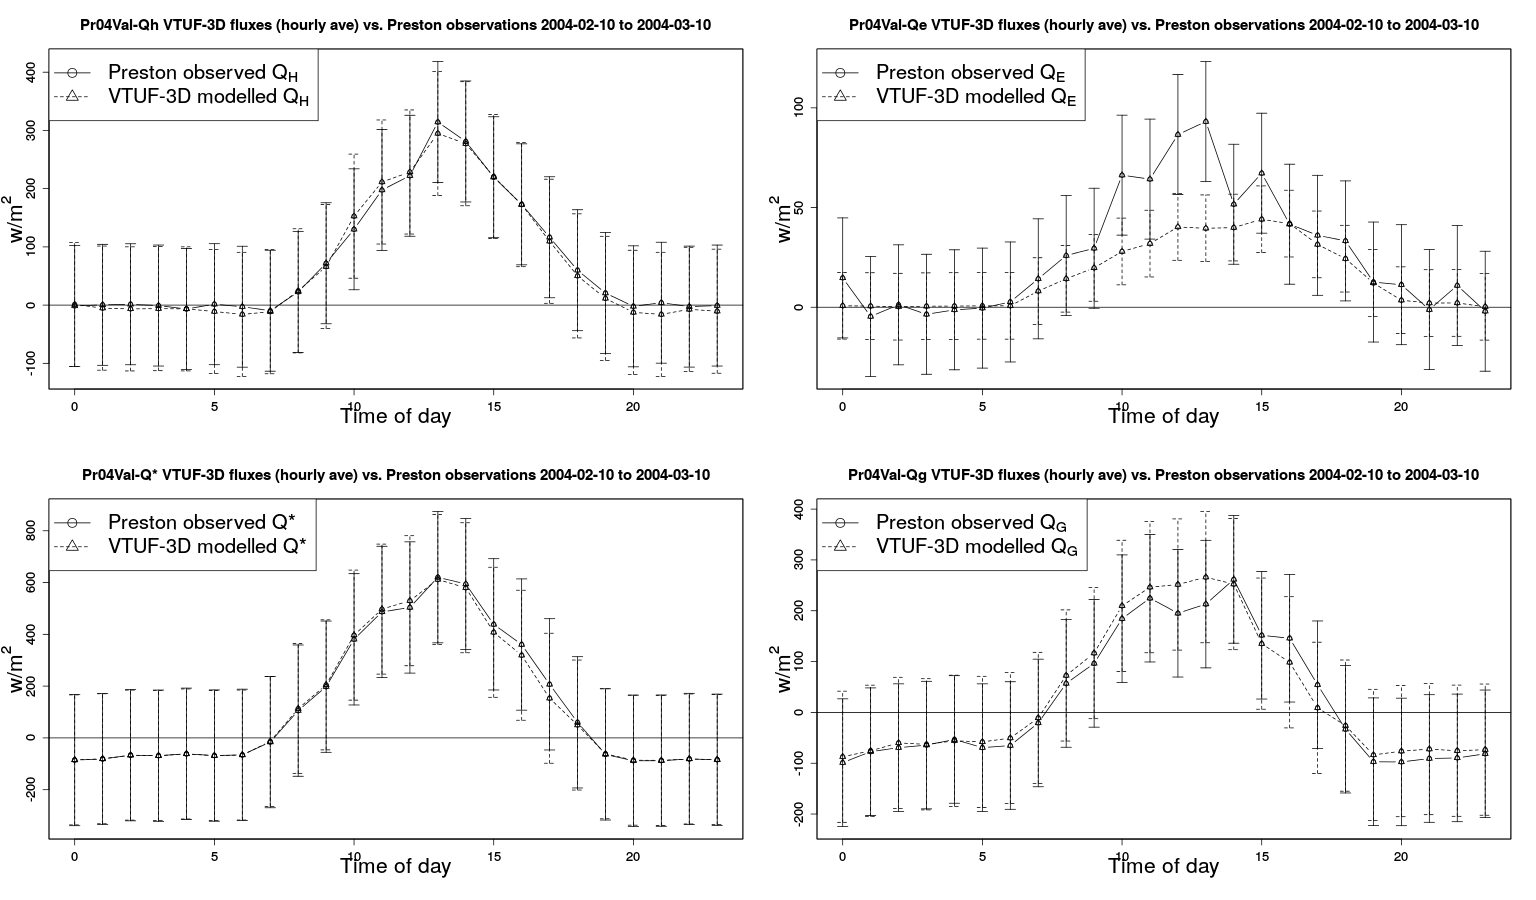
\includegraphics[trim = 0mm 0mm 0mm 0mm, clip, scale=0.30]{images/Pr04Val-EnergyBalanceOverallAve4Plots_.png}
\caption{Pr04Val run 30 day hourly average VTUF-3D flux comparisons to Preston flux observations for the period 10 February-10 March 2004, with error bars at standard deviations. \label{fig:Preston30Day4} }     
\end{figure}


In terms of absolute values, in 30 day monthly hourly averages, peaking daily values of $Q_{H}$ at 1300 are 314 W m$^{-2}$ in observed values compared to modelled values of 294. For the other fluxes, $Q_{E}$, $Q^{*}$, and $Q_{G}$, these values are 93 vs. 40, 621 vs. 612, and 213 vs. 266 W m$^{-2}$. An error analysis of d (index of agreement) for the Pr04Val validation (Figure 6) shows d values of 0.964, 0.652, 0.998, and 0.957 for $Q_{H}$, $Q_{E}$, $Q^{*}$, and $Q_{G}$ respectively. Error analysis of RMSE (W m$^{-2}$) shows values of 40.2, 33.1, 19.0,and 52.5. As an extension to the TUF-3D model, the addition of vegetation and associated $Q_{E}$ fluxes to VTUF-3D have created a large improvement to the model. As will be seen in the Intercomparison results (Section \ref{sec:interresults}), as well as in the results of this intercomparison project \citep{Grimmond2011,Best2012}, land surface modelling schemes that include vegetation perform better than those that do not. In addition, schemes that integrate vegetation perform better than those who use a tiling method to include the vegetation. Another important result from this intercomparison project is that $Q_{E}$ is the least well modelled flux across a range of urban land surface modelling schemes \citep{Grimmond2010}. Even the SUEWS model, which includes vegetation, as well as a very complete urban hydrology, tends to under-estimate $Q_{E}$ fluxes during day-time \citep{Jarvi2011}.


%During this validation, a number of different scenarios (described in Table \ref{tab:simscompared}) are considered and compared. The validation scenario (named Pr04Val) compares the mo the closest approximation of a domain (at a micro-scale) which could be constructed to match the local scaled flux observations. 

%The first result is given in Figure \ref{fig:Preston6error}. Modelled results for the 30 day run are compared to the observed fluxes ($Q^{*}$, $Q_{H}$, $Q_{G}$, and $Q_{E}$). Error analysis of d index of agreement for the Pr04Val validation (Figure \ref{fig:Preston6error}) shows d values of 0.964, 0.652, 0.998, and 0.957 for $Q_{H}$, $Q_{E}$, $Q^{*}$, and $Q_{G}$ respectively. Error analysis of $RMSE$ (W m$^{-2}$) shows values of 40.2, 33.1, 19.0,and 52.5. 


\begin{figure}[!htbp]
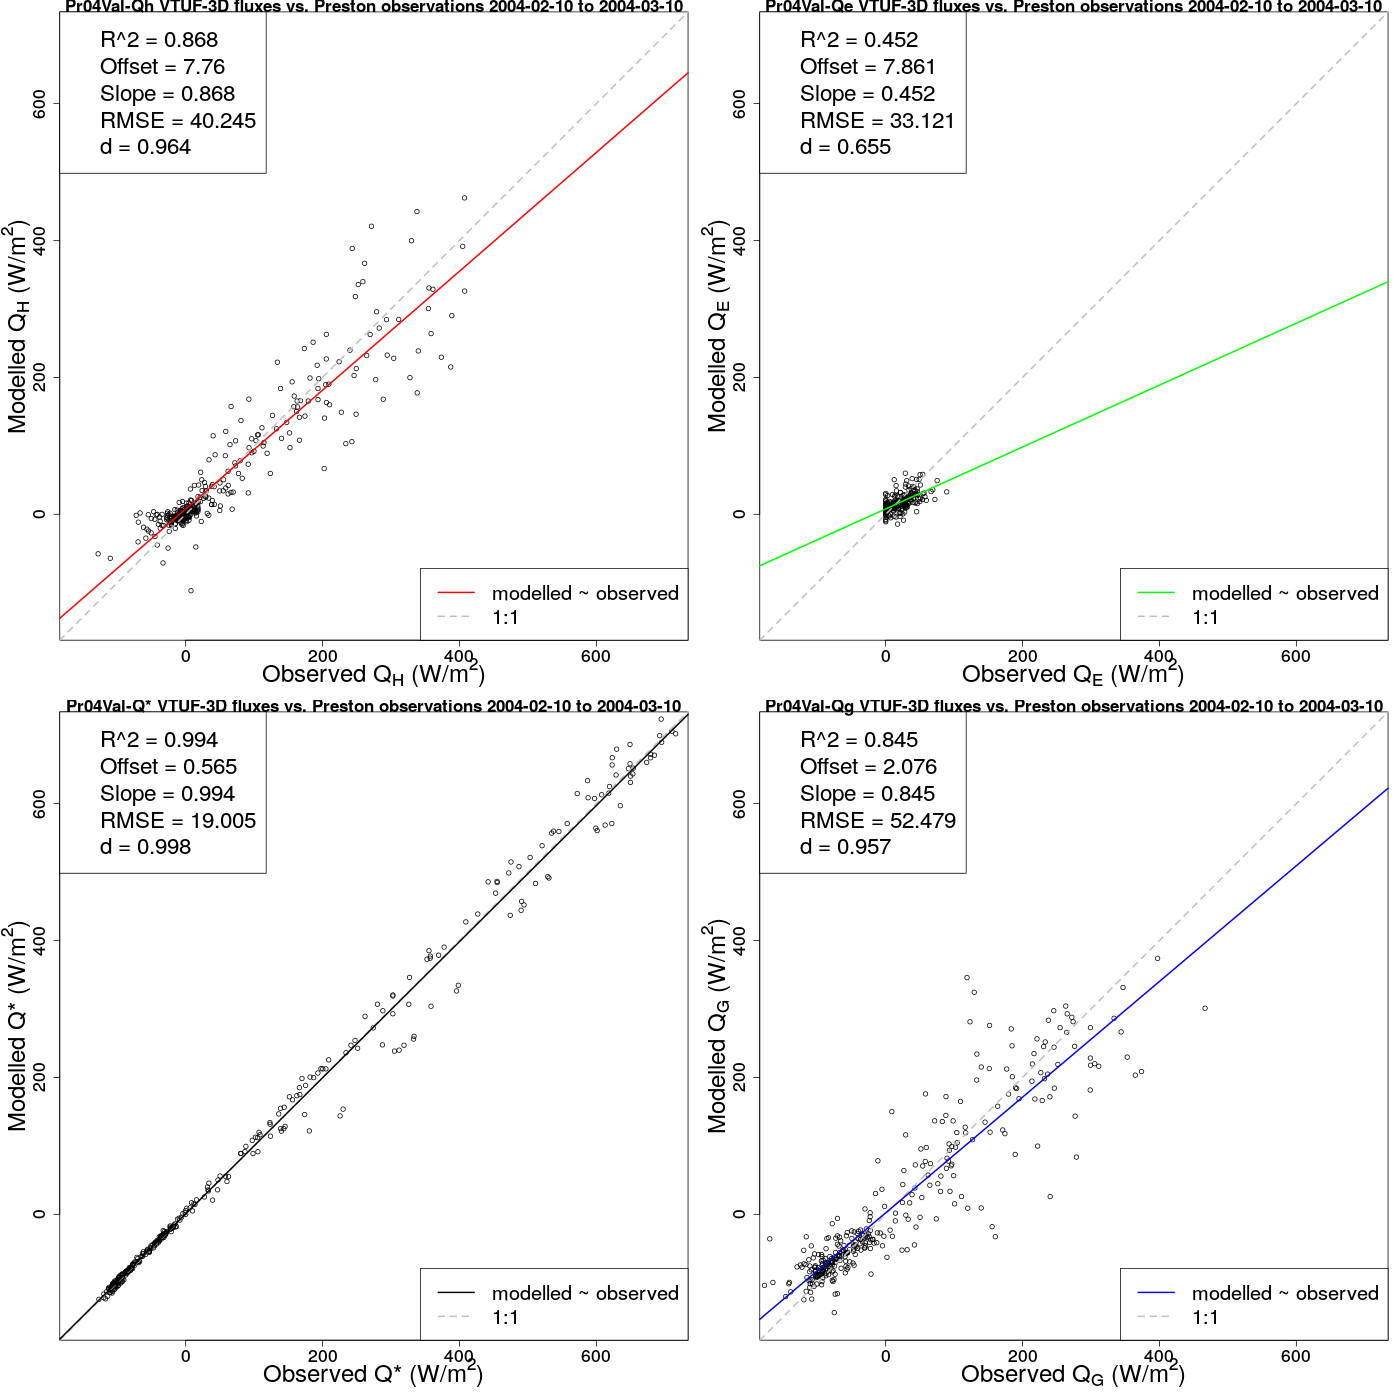
\includegraphics[trim = 0mm 0mm 0mm 0mm, clip, scale=0.30]{images/Pr04Val-ErrorPlots.png}
\caption{Pr04Val scenario modelled vs. observations for $Q_{H}$, $Q_{E}$, $Q^{*}$, and $Q_{G}$ fluxes for the period 10 February-10 March 2004. \label{fig:Preston6error}}   
\end{figure}

%Individual fluxes ($Q^{*}$, $Q_{H}$, $Q_{G}$, and $Q_{E}$) were aggregated into hourly averages over the 30 days and compared to the observations (Figure \ref{fig:Preston30Day4}). VTUF-3D is able to reproduce the important dynamics of this area, driven by the fluxes. In the observations, the $Q_{H}$ and $Q_{G}$ fluxes dominate the urban area, with modest amounts of $Q_{E}$ fluxes, peaking under 100W m$^{-2}$ during the daytime and falling to roughly zero at night-time. 

%\begin{figure}[!htbp] 
%\includegraphics[trim = 0mm 0mm 0mm 0mm, clip, scale=0.30]{/home/kerryn/Documents/Work/VTUF-Runs/PrestonBase/Analysis/Pr04Val-EnergyBalanceOverallAve_.png}
%\caption{Pr04Val run 30 day hourly average VTUF-3D flux comparisons to Preston flux observations for the period 10 February-10 March 2004, with error bars at observations standard deviations. \label{fig:Preston30Day}}      
%\end{figure}


%VTUF-3D captures closely both the magnitude and diurnal cycle of $Q_{H}$, with a slight under-prediction during the morning and a slight over-prediction during the late mornings. VTUF-3D also captures closely the cycles of $Q^{*}$. The very small divergence between the predicted and observed values can be explained through the dual sources of values of $K\downarrow$ in the forcing data, a distance of approximately 20 km between Preston and the Melbourne Airport observation site, providing varying values as a component of the calculated $Q^{*}$ which are then compared to only the Preston observations. $Q_{G}$ shows close agreement except for a slight over-prediction during the mornings, an over-prediction at mid-day, a slight over-prediction during the afternoon cooling period, and a very slight over-prediction during the evening.

%In terms of absolute values, in 30 day monthly hourly averages, peaking daily values of $Q_{H}$ at 1300 are 314 W m$^{-2}$ in observed values compared to modelled values of 294. For the other fluxes, $Q_{E}$, $Q^{*}$, and $Q_{G}$, these values are 93 vs. 40, 621 vs. 612, and 213 vs. 266 W m$^{-2}$.

%As an extension to the TUF-3D model, the addition of vegetation and associated $Q_{E}$ fluxes to VTUF-3D have created a large improvement to the model. As will be seen in the Intercomparison results (Section \ref{sec:interresults}), as well as in the results of this intercomparison project \citep{Grimmond2011,Best2012}, land surface modelling schemes that include vegetation perform better than those that do not. 

%In addition, schemes that integrate vegetation perform better than those who use a tiling method to include the vegetation. Another important result from this intercomparison project is that $Q_{E}$ is the least well modelled flux across a range of urban land surface modelling schemes \citep{Grimmond2010}. Even the SUEWS model, which includes vegetation, as well as a very complete urban hydrology, tends to under-estimate $Q_{E}$ fluxes during day-time \citep{Jarvi2011}.

It is anticipated that the innovative method taken in this project, the first time vegetation has been tiled and incorporated into a micro-scaled surface energy balance model, will bring performance improvements over the previous version of the model which did not consider vegetation. This will be seen to be the case, shown in the the results of the Pr04NoVeg no vegetation validation scenario (Section \ref{sec:baselinenoveg}). In addition to the improved modelling performance, the addition of vegetation modelling has dramatically improved the applicability of VTUF-3D to a wide range of modelling problems. Indeed, without this addition, the main aim of this model, to determine the thermal comfort improvements due to urban vegetation and water would not be possible. 

Despite these improvements to the modelling tool, the fluxes of $Q_{E}$ show some divergences from the observations. This was anticipated as there are three current limitations of VTUF-3D that can account for low $Q_{E}$ levels, and need addressing in future versions of the model. The first is not accounting for precipitation on impervious surfaces. Many spikes of $Q_{E}$ fluxes are seen in the observations shortly after rainfall. \cite{Demuzere2014} found evaporation from impervious surfaces in urban areas after rainfall can contribute to an approximately 10\% increase of $Q_{E}$ over a two month period, while \cite{Wouters2013} found increases of 45 W m$^{-2}$ in $Q_{E}$ for up to 12 hours of daylight following rainfall. Until this portion of precipitation received is accounted for in the model, care should be taken when modelling periods which contain precipitation.

%\begin{figure}[!htbp] 
%\includegraphics[trim = 0mm 0mm 0mm 0mm, clip, scale=0.30]{/home/kerryn/Documents/Work/VTUF-Runs/PrestonBase/Analysis/Pr04Val-QeTimeseries.png}
%\caption{Pr04Val modelled $Q_{E}$ vs. Preston $Q_{E}$ observations including observation of daily high/low temperatures and hourly rain totals for the period 10 February-10 March 2004. \label{fig:Preston30DayQe} }     
%\end{figure}

The second limitation is not accounting for irrigation. While Melbourne was under Stage 2 water restrictions during the observation/modelling period \citep{MelbourneWater2016a}, there would have been some amount of irrigation occurring to contribute to greater observed $Q_{E}$ fluxes than modelled. Estimates of household irrigation during February 2004 are of frequencies of 2.8 times a week (3.1 for only the homes which irrigate) with average irrigation flows of 16.3 LpM and average durations of 46 minutes per irrigation event \citep{Roberts2005}. This is an important limitation which needs addressing as quantifying the benefits of irrigation as part of WSUD is an intended use of this model. The third limitation is the full diversity of vegetation and trees of the modelled area are not represented in the modelled domain. In this study, parametrisations were included for grass, brushbox, and olive trees. However, this is not a limitation in the model itself, as any type of vegetation can be plugged into the model. To overcome this deficit, more work needs to be done. Completion of each parametrisation is a time consuming process requiring numerous observations of tree physiology specifications. A standard limitation of many empirical models requiring a choice of either deciduous or evergreen vegetation does not exist in the model itself as these new vegetation types can include either, as long as the proper observations and parametrisations are completed on each type.


Another consideration is that the under-prediction of $Q_{E}$ is likely contributing to the over-estimating of $Q_{G}$ (calculated as a residual in MAESPA vegetation tiles). An improvement in modelling of the $Q_{E}$ fluxes will likely lead to an improvement in the modelled $Q_{G}$ fluxes. Finally, values of $Q_{F}$, anthropogenic heat (W m$^{-2}$), are not accounted for in the VTUF-3D model, but which do contribute to the total $Q_{H}$ fluxes in the observations. Flux values for this modelling and observation period (summertime) are anticipated to contribute peaks of over 15 W m$^{-2}$ for low density areas of cities and peaks of 30-60 W m$^{-2}$ for medium density areas \citep{Sailor2004}. In both the observations and modelling results, these unaccounted fluxes will be present in the errors for the four observed and modelled fluxes.

There will remain an amount of uncertainty in comparing the modelled results to the observations because of the nature of both. The observations were collected via a flux tower at 40m height, above the height of the urban roughness sublayer. The modelled results are the average of the fluxes from all of the urban surfaces, within the urban canyon and well within the urban roughness sublayer. While these comparisons can be done, i.e. \cite{Grimmond2011}, there remains an amount of uncertainly as they are comparing two slightly different things. 



\subsection{No vegetation scenario}\label{sec:baselinenoveg}

%To demonstrate the significant improvement of the model, the VTUF-3D model was run with a no vegetation scenario. This scenario (named Pr04NoVeg), will represent an unimproved TUF-3D without vegetation modelling capability, as the lack of vegetation will not trigger any of the new logic and improvements added to the model. This will allow an analysis of level of improvement of VTUF-3D modelling over the previous TUF-3D model. As discussed earlier in this section, the Intercomparison project found that models without vegetation were among the poorest performers.
 
Figure \ref{fig:Prestonnoveg30day} presents a 30 day hourly average of both the Pr04Val and Pr04NoVeg scenarios with the Pr04Val showing a much closer fit for all fluxes over a diurnal cycle. Figure \ref{fig:Prestonnovegerror} presents each component of the surface energy balance for the no vegetation scenario (Pr04NoVeg). These values show an improvement over the unimproved VTUF-3D model. The unimproved model yields results of d of 0.906, 0.0, 0.989, and 0.877 and $RMSE$ (W m$^{-2}$) of 87.0, 47.1, 51.6, 75.9 for $Q_{H}$, $Q_{E}$, $Q^{*}$, and $Q_{G}$ respectively. As an unimproved model, $Q_{H}$ is significantly over-predicted during the afternoon and under-predicted in the evenings. Flux $Q_{G}$ is under-predicted during the afternoons. Finally, $Q_{E}$ is not implemented in the model, so cannot be predicted at all. 


\begin{figure}[!htbp]
\includegraphics[trim = 0mm 0mm 0mm 0mm, clip, scale=0.16]{images/Pr04Val-EnergyBalanceOverallAve_.png}
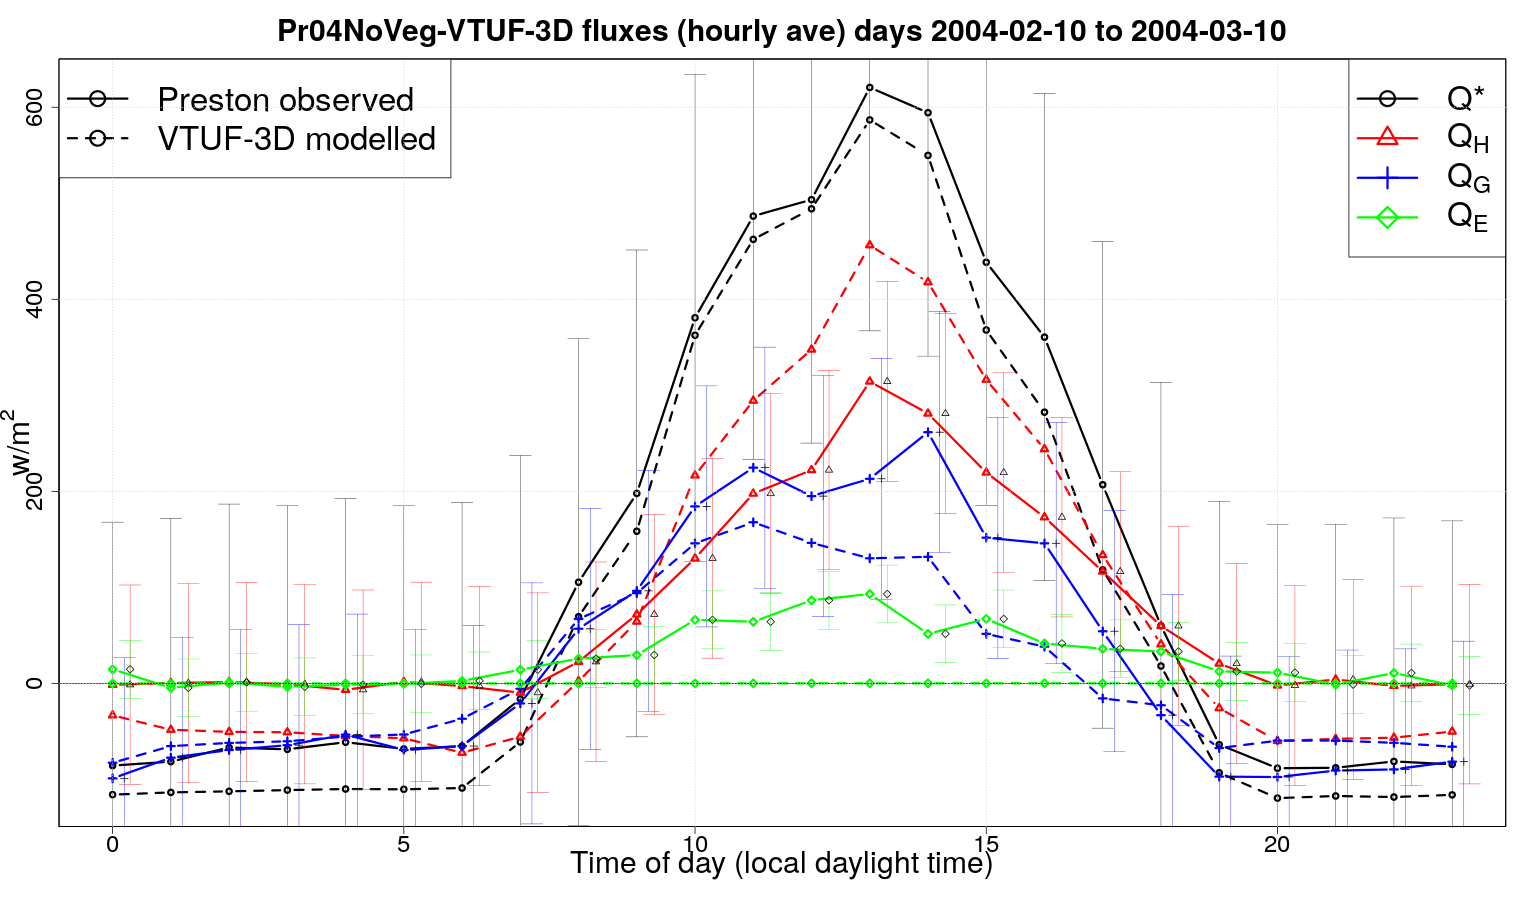
\includegraphics[trim = 0mm 0mm 0mm 0mm, clip, scale=0.16]{images/Pr04NoVeg-EnergyBalanceOverallAve_.png}
\caption{Pr04Val and Pr04NoVeg scenarios. 30 day hourly average VTUF-3D flux comparisons to Preston flux observations for the period 10 February-10 March 2004, with error bars at observations standard deviations. \label{fig:Prestonnoveg30day}}    
\end{figure}

\begin{figure}[!htbp]
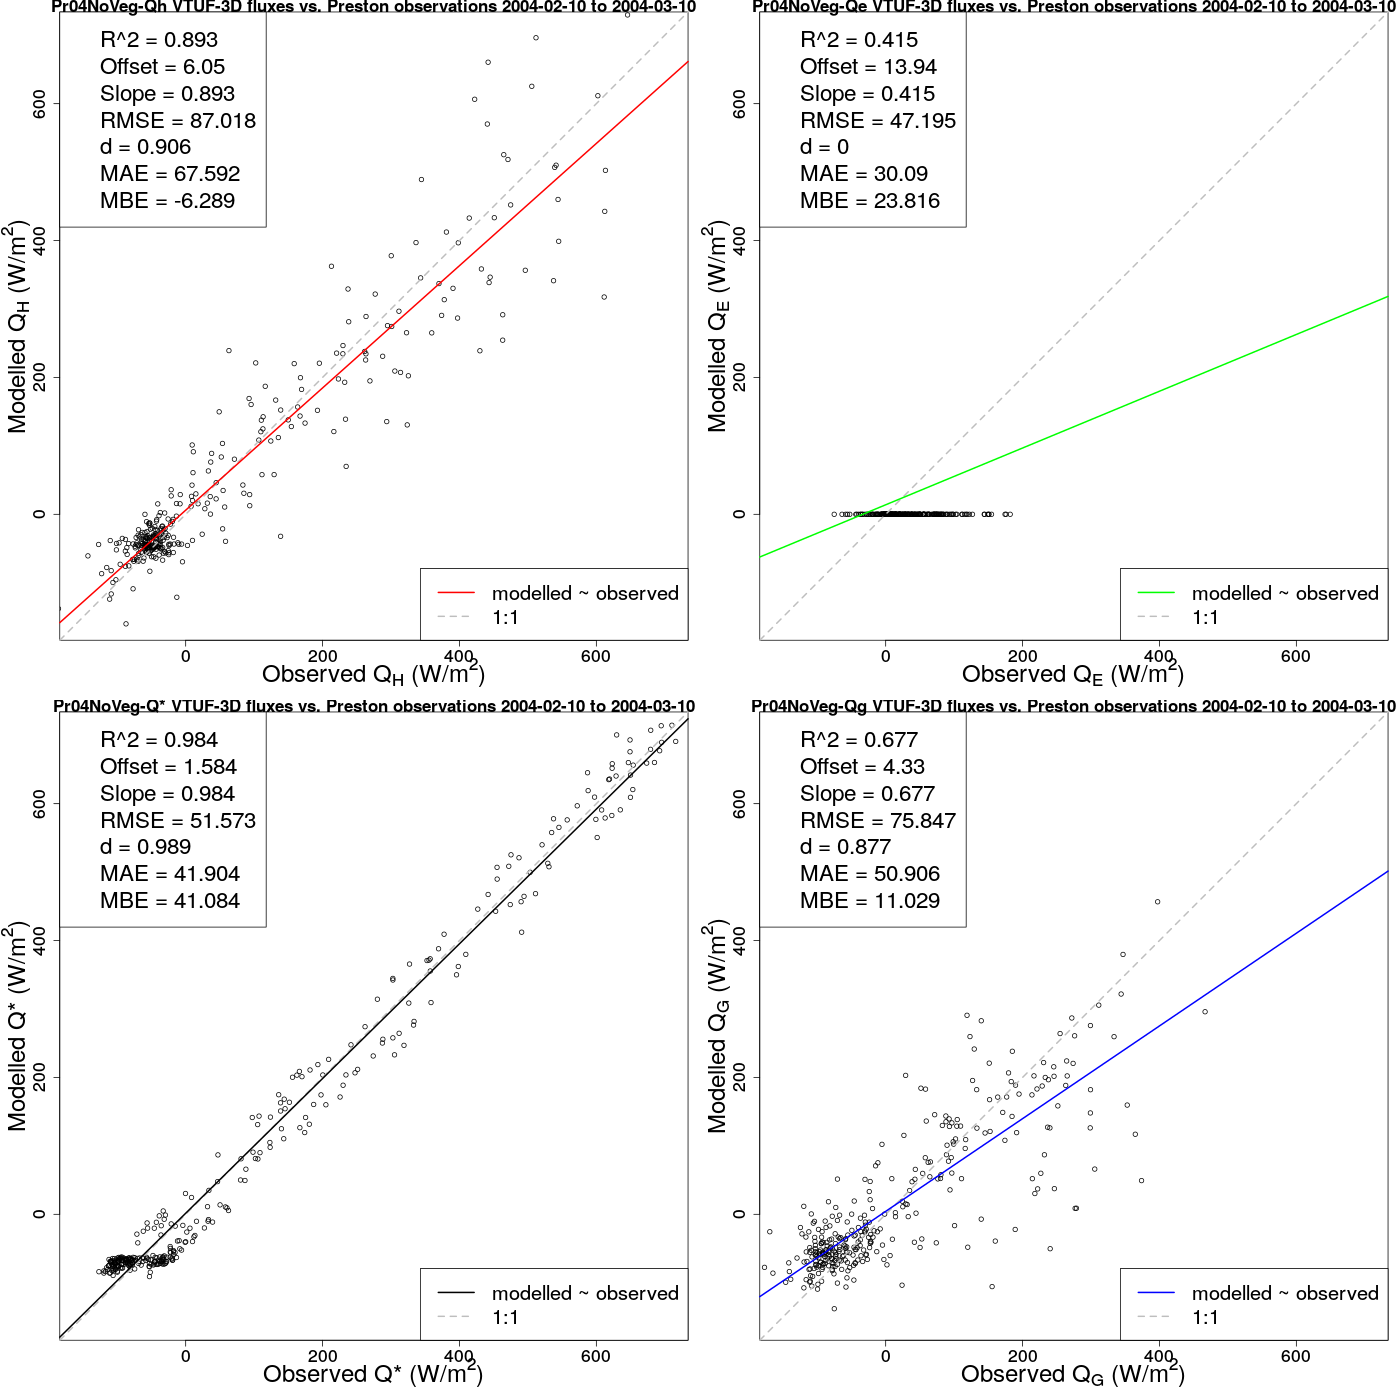
\includegraphics[trim = 0mm 0mm 0mm 0mm, clip, scale=0.30]{images/Pr04NoVeg-ErrorPlots.png}
\caption{Pr04NoVeg scenario modelled vs. observations for $Q_{H}$, $Q_{E}$, $Q^{*}$, and $Q_{G}$ fluxes for the period 10 February-10 March 2004. \label{fig:Prestonnovegerror}}    
\end{figure}




\subsubsection{Preston validation intercomparison results and discussion}\label{sec:interresults}
%During this validation, a number of different scenarios are considered and compared. The Pr04Val scenario (a scenario to best represent the area observed by the Preston flux tower observations) is compared to a baseline Pr04NoVeg scenario (an unimproved TUF-3D without vegetation modelling capability). As the observations used in this validation are the same as in Phase 4 of the Intercomparison project \citep{Best2012}, using the \cite{Coutts2007} Preston dataset, the performance of the VTUF-3D model can also be placed within this evaluation of urban land surface modelling schemes. 

%Intercomparison Phase 4 error analysis provides $RMSE$ values for fluxes $Q^{*}$, $Q_{H}$, $Q_{G}$, and $Q_{E}$ for three classifications of urban models. These three categories are of models that do not consider vegetation, those that model vegetation using tiles, and models that integrate vegetation into the urban area (referred to as classifications IntercomparisonNoVeg, IntercomparisonTiled, and IntercomparisonIntegrated, described in Table \ref{tab:simscompared}). 

Using the RMSE values for fluxes $Q^{*}$, $Q_{H}$, $Q_{G}$ from Phase 4 of the Intercomparison project, the performance of the Pr04NoVeg scenario (as well as the Pr04NoVeg scenario) can be compared against the performance of 24 other urban land surface models. The RMSE values are taken from Figure 2 of \cite{Best2012}, for the Feb/Mar period, corresponding to the period for which the validation scenarios were run. 

%\begin{figure}[!htbp]
%\includegraphics[trim = 0mm 18mm 00mm 0mm, clip, scale=0.80]{/home/kerryn/git/Images/Best2012-Fig2-IntercomparionsRMSE.png} \caption{Median of the mean modelled flux, MBE, and RMSE for the surface fluxes determined for two month periods, for the models classified by their representation of vegetation. Note the scales are different for each flux \citep{Best2012}. \label{fig:best2012RMSE}}  
%\end{figure}

%\begin{figure}[!htbp] 
%\includegraphics[trim = 0mm 0mm 0mm 0mm, clip, scale=0.25]{/home/kerryn/Documents/Work/VTUF-Runs/PrestonBase/Analysis/IntercomparisonIntegrated-ErrorPlotsRMSECombined2.png}
%\caption{RMSE VTUF-3D vs. Intercomparison results comparison for Preston validations scenarios for 10 February-10 March 2004.\label{fig:prestonrmse}}      
%\end{figure}

A comparison of Intercomparison RMSE results vs. modelled results is shown in Table \ref{fig:prestonrmse}. In Phase 4 comparisons, for all fluxes, models with integrated vegetation had the lowest $RMSE$ values. These were followed by tiled vegetation models while models without vegetation had the highest values. In comparison, the VTUF-3D Pr04Val scenario had lower $RMSE$ values for all fluxes except $Q_{E}$ than each of the Phase 4 three model categories. For $Q_{E}$, the VTUF-3D scenario Pr04Val performed better than the no vegetation category, but with slightly higher errors than the tiled and integrated categories. In terms of absolute differences between $RMSE$ values for the best performing Intercomparison model category, Pr04Val scenario $RMSE$ values differed by -6, -5, -25, and 7 W m$^{-2}$ for $Q^{*}$, $Q_{H}$, $Q_{G}$, and $Q_{E}$ respectively.

\begin{center}
\begin{table}[!htbp]
\caption{RMSE VTUF-3D vs. Intercomparison results \citep{Best2012} comparison for Preston validations scenarios for 10 February-10 March 2004.\label{fig:prestonrmse}} 
\begin{tabular}{  | l | l | l|l|l| } 
\hline \textbf{Scenario name} &\textbf{$Q^{*}$}& \textbf{$Q_{H}$}& \textbf{$Q_{G}$}& \textbf{$Q_{E}$}  \\ \hline
Pr04Val & 19.0&	40.2&	52.5&	33.1    \\ \hline
Pr04NoVeg & 51.6&	87.0&	75.9&	47.1  \\ \hline	
IntercomparisonNoVeg & 40&	105&	85&	38   \\ \hline
IntercomparisonTiled &  27&	60&	77&	25  \\ \hline
IntercomparisonIntegrated & 25&	45&	77&	26   \\ \hline
  \end{tabular} 
\end{table}
\end{center} 



\section{Summary and Conclusions}

This study presents the development of a new model, VTUF-3D, that is able to model vegetation and WSUD features, accounting for latent energy fluxes and their impacts on HTC. Two major modifications were made to the original TUF-3D model in the development of VTUF-3D. The first major modification added physical representations of vegetation and allow the shading effects of these features to be modelled. The second major modification added the ability to model vegetation physiological processes (and associated water cycles). These modifications allow surface energy balances to be repartitioned, accounting for latent energy fluxes, as well as the effects that vegetation shading will have on these energy balances.

This analysis of VTUF-3D performance when comparing predicted results to flux tower observations and in comparison to error rates of other urban models has shown significant improvement over the unimproved (non-vegetated) TUF-3D model. Furthermore, these comparisons to observations show the model is able to capture well the temporal and amplitude variations of fluxes observed by flux towers. In a comparison of VTUF-3D modelled results to other types of urban land surface schemes, VTUF-3D performs well within the range of those other models, even though most of those models are local scaled and not being run at a micro-climate scale. Error analysis puts VTUF-3D's performance in all fluxes, except $Q_{E}$, as slightly better than all categories of these models. With the $Q_{E}$ flux, VTUF-3D performs with lower error rates than the models in the no vegetation category but with slightly higher errors than in the tiled and integrated categories. This validation demonstrates that VTUF-3D performs well in terms of surface energy balances, lending weight to its suitability to assess the impacts of urban greenery on human thermal comfort. Two further validations focussing on urban canopy layer air temperature and the Universal Thermal Climate Index (to be detailed in a forthcoming paper), will add additional confidence to VTUF-3D's suitability to accurately model urban areas and urban vegetation.

VTUF-3D is a unique model involving an innovative tiling approach that accounts for the detailed physiological processes of vegetation. The model incorporates a templated scalable configuration system, used to represent specific types of vegetation, allowing any variety and mix of vegetation to be added to a modelled domain. Also, differential shading functionality allows impacts of urban geometry and inter-tree shading on vegetation anywhere in an urban canyon to be properly modelled. Finally, the addition of mean radiant temperature and UTCI output for all surfaces allows detailed analysis of the impact of vegetation on these important parameters influencing HTC in these areas.

An extensive validation process has shown that VTUF-3D is able to accurately model urban areas (including urban vegetation). Now, with the completion and validation of the VTUF-3D v1.0 model, there is a suitable tool to model and study in detail the impacts of urban greening on HTC and recommendations and guidelines on how to best use urban greenery can be developed. Questions can be answered as to the optimal arrangement of canopy cover to give the maximum benefits. Performance of future scenarios can also help inform responses to future challenges, both in terms of urban redesign and planning for emergency responses.

With VTUF-3D's micro-climate resolution, urban areas can be studied metre by metre and proper mitigation strategies designed for every section of the urban canyon, allowing effort to be focused on areas with the greatest need. VTUF-3D is sufficiently scaled to resolve human level interactions with their surroundings and provide variables to calculate HTC (such as T$_{mrt}$). The built in output of T$_{mrt}$ and UTCI allows examination of these values without requiring addition steps. Finally, with the ability to insert any type of vegetation using physiological and physical vegetation templates, VTUF-3D is applicable to an unlimited number of scenarios and modelling questions. This new model will allow research into a wide variety of urban morphologies, quantifying the benefits of a wide variety of urban arrangements and allow planning for future changes and challenges in climate and urban design.

%This analysis of VTUF-3D performance when comparing predicted results to flux tower observations and in comparison to error rates of other urban models has shown significant improvement over the unimproved (non-vegetated) TUF-3D model. Furthermore, these comparisons to observations show the model is able to capture well the temporal and amplitude variations of fluxes observed by flux towers. 
%
%In a comparison of VTUF-3D modelled results to other urban models, VTUF-3D performs well within the range of those other models, even though most of those models are local scaled and not being run at a micro-climate scale. Error analysis puts VTUF-3D's performance in all fluxes except $Q^{*}$ slightly better than the all categories of these models. With the $Q^{*}$ flux, VTUF-3D performs with lower errors than the models in the no vegetation category but with slightly higher errors than in the tiled and integrated categories. 
%
%This validation demonstrates that VTUF-3D performs well in terms of surface energy balances, lending weight to its suitability to assess the impacts of urban greenery on human thermal comfort. Two following validations (to be detailed in a forthcoming paper), will add additional confidence to VTUF-3D's suitability to accurately model urban areas and urban vegetation.
%
%
%\section{Conclusions} \label{sec:DesignConc} 
%
%These modifications to TUF-3D have created a new model, VTUF-3D, able to model vegetation, account for latent energy fluxes, and shown suitable to model WSUD features and their HTC impacts. Two major modifications were made to create VTUF-3D. The first added physical representations of vegetation and allow the shading effects of these features to be modelled. The second added the ability to model vegetation physiological processes (and associated water cycles). These modifications allow surface energy balances to be repartitioned, accounting for latent energy fluxes, as well as the effects that vegetation shading will have on these energy balances. 
%
%A templated scalable configuration system, used to represent arbitrary types of vegetation (or other WSUD features), allows any variety and mix of vegetation to be added to a modelled domain. Also, differential shading functionality allows impacts of urban geometry and inner tree shading on vegetation anywhere in an urban canyon to be properly modelled. Finally, the addition of mean radiant temperature and UTCI output for all surfaces allows detailed analysis of the vegetations impact on these important parameters on HTC in these areas.
%
%An extensive validation process has shown that VTUF-3D is able to accurately model urban areas (including urban vegetation). Now, with the completion and validation of the VTUF-3D v1.0 model, there is a suitable tool to model and study in detail the impacts of urban greening on HTC and recommendations and guidelines on how to best use urban greenery can be developed. Questions can be answered as to the optimal arrangement of canopy cover to give the maximum benefits. Performance of future scenarios can also help inform responses to future challenges, both in terms of urban redesign and planning for emergency responses.
%
%With the VTUF-3D's micro-climate resolution, urban areas can be studied metre by metre and proper mitigation strategies designed for every section of the urban canyon, allowing effort to be focused on areas with the greatest need.  It is sufficiently scaled to resolve human level interactions with their surroundings and provide variables to calculate HTC (such as $T_{mrt}$). The built in output of $T_{mrt}$ and UTCI allows examination of these values without requiring addition steps. Finally, with the ability to insert any type of vegetation (or WSUD feature) using physiological and physical vegetation templates, VTUF-3D is applicable to an unlimited number of scenarios and modelling questions. This new model will allow research into a wide variety of urban morphologies, quantifying the benefits of a wide variety of urban arrangements and allow planning for future changes and challenges in climate and urban design.



\section{Code availability}\label{sec:available}

Development of VTUF-3D was conducted in FORTRAN 2003 \citep{GNU2016a} in Netbeans 8.0.2 \citep{Netbeans2016} and compiled with gfortran 4.8.4 \citep{GNU2016} on Ubuntu 14.04, however, the code should compile on any platform with FORTRAN 2003 support. The original source code for TUF-3D was obtained from the author \citep{Krayenhoff2007}, while source code for MAESPA was obtained from the MAESPA repository \citep{Duursma2016}. The development process merged these code bases and added the additional functionality described in this paper. The VTUF-3D source code is available at \cite{Nice2016c}.

Model configuration process was developed in Java using the JRE 1.7.0 \citep{Oracle2016} in Eclipse 4.5.2 \citep{Eclipse2016}. Data analysis and graphing scripts were generated in R \citep{R2013} and Python \citep{Python2016} using the Matplotlib library \citep{Hunter2007}. 


\section{References}\label{sec:ref}
%% If you have bibdatabase file and want bibtex to generate the
%% bibitems, please use
%%
  \bibliographystyle{elsarticle-harv} 
  \bibliography{library}

%% else use the following coding to input the bibitems directly in the
%% TeX file.

\begin{thebibliography}{00}

%% \bibitem[Author(year)]{label}
%% Text of bibliographic item

\bibitem[ ()]{}

\end{thebibliography}


%% The Appendices part is started with the command \appendix;
%% appendix sections are then done as normal sections
\appendix


%\subsection{}                               %% Appendix A1, A2, etc.


%%%%%%%%%% taking out parameterizations
\section{MAESPA vegetation parameterisations}\label{sec:maespavegpara}  
%
%The physiological properties of the two selected trees and grass were integrated into the configuration files. All parameterisations used in this study share some common attributes, summarised in Table \ref{tab:commonattr}.
%
%\begin{table}[!htbp]
%\caption{MAESPA tree parameterisations common attributes. \label{tab:commonattr}} 
%\begin{tabular}{ |  p{13cm} | p{4cm} |}
%\hline \textbf{Parameter} & \textbf{Value}  \\ 
%\hline
%Stomatal conductance model & Ball-Berry-Opti model \citep{Medlyn2011} \\ \hline
%Number of layers in the crown assumed when calculating radiation interception &6	 \\ \hline
%Number of points per layer&12 \\ \hline
%Number of zenith angles for which diffuse transmittances are to be integrated &5   \\ \hline
%Number of azimuth angles for which diffuse transmittances are to be integrated&11  \\ \hline
%\end{tabular} 
%\end{table}
%
\subsection{MAESPA olive tree (\textit{Olea europaea}) parameterisation}
The first complete parameterisation for VTUF-3D is the olive tree (\textit{Olea europaea}). It has been selected because it is a species commonly found in gardens in Melbourne, considered suitable for Melbourne's climate conditions (drought tolerant evergreen), and a recommended species for council street tree planting \citep{PortPhillip2010}. In addition, observations of parameters are available from \cite{Coutts2014a}. The physical and meteorological parameters for a 5x5 meter grid square are given in Table \ref{tab:olivescaled}. 

\begin{center}
\begin{table}[!htbp]
\caption{MAESPA olive tree (\textit{Olea europaea}) parameterisation, tree dimensions for an example 5x5m grid (to be rescaled for taller/shorter modelled trees).\label{tab:olivescaled}}
\begin{tabular}{ |  l | l | l | l |}
\hline \textbf{Parameter} & \textbf{Value} & \textbf{Source} \\ 
\hline
crown radius (m) & 2.5 & \cite{Coutts2014a}\\ \hline
crown height (m) & 3.75 & \cite{Coutts2014a}\\ \hline
trunk height (m) & 1.25 & \cite{Coutts2014a}\\ \hline
leaf area index (m$^{2}$ m$^{-2}$)&2.48 &\cite{Mariscal2000}\\ \hline
crown shape & round &\\ \hline
$z_{Ht}$ (m)&40.0&Forcing data height \\ \hline
$z_{PD}$ (m) &2.5& 2/3 of crown height `rule of thumb' \citep{Grimmond1999}\\ \hline
$z_{0,Ht}$ (m) &0.375& 1/10 of crown height `rule of thumb' \citep{Grimmond1999} \\ \hline
\end{tabular} 
\end{table}
\end{center}

\begin{center}
\begin{table}[!htbp]
\caption{MAESPA olive tree (\textit{Olea europaea}) parameterisation, with parameter values taken from cited literature sources. \label{tab:oliveparam}}

\scalebox{0.85}{
\begin{tabular}{ |  p{9.3cm} | p{2.5cm} | p{5.6cm} |}
\hline \textbf{Parameter} & \textbf{Value(s)} & \textbf{Source} \\ 
\hline
Soil reflectance (\%PAR, \%NIR, and \%IR)  & 0.10, 0.05, 0.05 & \cite{Levinson2007,Oke1987z} \\ \hline
Leaf transmittance (\%PAR, \%NIR, and \%IR)  & 0.01, 0.28, 0.01 & \cite{Baldini1997} \\ \hline
Leaf reflectance (\%PAR, \%NIR, and \%IR)  & 0.08, 0.42, 0.05 & \cite{Baldini1997} \\ \hline
Minimum stomatal conductance g0 (mol m$^{-2}$s$^{-1}$) & 0.03 & \cite{Coutts2014a}\\ \hline
Slope parameter g1  & 2.615 &\cite{Coutts2014a} \\ \hline
\# of sides of the leaf with Stomata & 1&\cite{Fernandez1997}\\ \hline
Width of leaf (m)& 0.0102&\\ \hline
CO$_{2}$ compensation point ($\mu$mol m$^{-2}$s$^{-1}$)& 55& \cite{Coutts2014a}\\ \hline
Max rate electron transport (Jmax) ($\mu$mol m$^{-2}$s$^{-1}$)& 112.4& \cite{Coutts2014a}\\ \hline
Max rate rubisco activity (VCmax) ($\mu$mol m$^{-2}$s$^{-1}$)& 81.18& \cite{Coutts2014a}\\ \hline
Curvature of the light response curve &0.62& \cite{Coutts2014a}\\ \hline
Activation energy of Jmax (KJ mol$^{-1}$)& 35350& \cite{Diaz-Espejo2006}\\ \hline
Deactivation energy of Jmax (J mol$^{-1}$)& 200000 &\cite{Medlyn2005a}\\ \hline
Entropy term (KJ mol$^{-1}$)& 644.4338& \cite{Medlyn2005a}\\ \hline
Quantum yield of electron transport (mol electrons mol$^{-1}$)& 0.19& \cite{Sierra2012}\\ \hline
Dark respiration ($\mu$mol m$^{-2}$s$^{-1}$)& 0.94& \cite{Coutts2014a}\\ \hline
Specific leaf area (mm$^{2}$kg$^{-1}$)&5.1 &\cite{Mariscal2000}\\ \hline
\end{tabular} 
}
\end{table}
\end{center}
%
%
%g0 = 0.03		!residual conductance/minimum stomatal conductance (mmol.m-1.s-1) (From Smith St. data)
%g1 = 2.615		!Slope parameter/coefficient (kPA^0.5) (From Smith St. data) (g1 must be for H2O of stomatal conductance)
%nsides = 1		!no. of sides of the leaf with Stomata
%wleaf = 0.0102		!width of leaf (metres)
%gamma = 55		!CO2 compensation point (CO2 curves)
%
%&jmax
%values = 112.4		!Value for Jmax (maximum rate of electron transport) (umol.m-2.s-1) (CO2 Curves)
%
%&vcmax
%values = 81.18		!Value for VCmax (maximal rate of rubisco activity at 25 degrees) (umol.m-2.s-1) (CO2 curves)
%
%	
%&jmaxpars
%theta =0.62		!Curvature of the light response curve of electron transport (PAR curves)
%eavj = 35350		!Activation energy of Jmax (KJ.mol-1) (also know as Hj) (Bernacchi et al 2001)
%edvj = 200000		!Deactivation energy of Jmax (J.mol-1) (Medlyn et al 2005)
%delsj = 644.4338	!Entropy term (KJ.mol-1)
%ajq = 0.19		!Quantam yield of electron transport (mol.mol-1) (PAR curves) (PSICO2=Absorb*8*0.5)
%/
%
%&rd
%values = 0.94		!Dark respiration (umol.m-2.s-1) (CO2 Curves)
%dates = '01/03/15' 	!Date for which Rd is specified
%/
%
%&sla
%values = 5.1		!Specific leaf area (5.1=Mariscal et al 2000) (m2.kg-1) Specific leaf area (SLA) is the one-sided area of a fresh leaf, divided by its oven-dry mass
%dates = '01/03/15'
%
%% tree.dat
%&aerodyn			
%zht = 4			!Height of wind speed measurements (Met file for Smith st used East Melbourne wind speed)
%zpd = 6.67		!2/3 of the tree crown height (rule of thumb)
%z0ht = 1		!1/10 of the tree crown height (rule of thumb)
%/
%leaf area (m2.tree-1)
%&alllarea		
%nodates = 1
%values = 48.7		!Total leaf area then is = LAI * tree area (radius^2*pi). LAI=2.48; 5^2*pi=19.6; => Total LA=48.7
%/
%
%%watpars.dat
%Single tree in Smith St Collingwood
%
%
%&watcontrol
%keepwet = 0		!Soil water stays wet if = 1 (used for testing)
%simtsoil = 1		!Simulate soil temperature (yes=1) (must do)
%simsoilevap = 1		!Simulate soil evaporation (yes=1)
%reassignrain = 0	!Re-assign half hourly rain if only DAILY rainfall (PPT) available (yes=1)
%wsoilmethod = 1		!If = 1 then use Emax method (unlimited water); if = 2 Use Vol Wat content; if = 4 use exponenetial relationship with SMD1 & SMD2;
%retfunction = 1		!Water retention curve (1=Campbell curve: parameters in "soilret")
%equaluptake = 0		!water uptake from soil layers (0=based on fine root density and soil water potential)
%usemeaset = 0		!Use canopy transpiration if = 1; need to add 'ET' to met.dat file
%usemeassw = 1		!Use measured soil water if = 1; 
%usestand = 0		!If = 1, water used by single trees scaled up to stand; If=0, scaling not done - use for single tree in stand, or BY ITSELF
%/
%
%Rainfall canopy interception
%&wattfall
%rutterb = 3.7		!Drainage coefficient (B parameter in Rutter et al 1975) to calculate canopy drainage (mm)
%rutterd = 0.002		!Drainage parameter in Rutter et al 1975 (0.002) (dimensionless)
%maxstorage = 0.4	!Maximum canopy storage of water
%throughfall = 0.6	!rainfall passing through the canopy
%/
%
%&watinfilt
%expinf = 0.0		!
%/
%
%Soil evaporation
%&soiletpars
%drythickmin = 0.01	!Minimum thickness of the dry soil layer (m)
%tortpar = 0.66		!XX Parameter describing tortuosity of the soil: describes diffusion in porous media
%/
%
%Root parameters
%&rootpars
%rootrad = 0.0001	!Average root radius (m)
%rootdens = 0.5e6	!Root density (g.m-3)
%rootmasstot = 2.4	!Total root biomass (kg.m-2) (0.417*d^2 where d is trunk diameter Ruiz-Peinado et al 2012)
%nrootlayer = 7		!Number of soil layers that are rooted. Together with the LAYTHICK parameter, it determines the rooting depth
%rootbeta = 0.9		!Beta parameter characterising root distribution (Jackson et al 1996)
%/
%
%Plant parameters
%&plantpars 
%minrootwp = -2.5	!Minimum root water potential (MPa) (Fernandez and Moreno 2008)
%minleafwp = -10		!Minimum leaf water potential (MPa) (not needed if MODELGS=6: Tuzet model) (Giorio 1999)
%plantk = 1.8		!leaf specific (total) plant hydraulic conductance (IMPORTANT!!!) (Dichio et al 2013) (=3.21 kg.m-2.s-1.MPa-1 x 10^-5   divide by 1.8 x 10^-5 gives 1.8 mmol.m-2.s-1.MPa-1)
%/
%
%Soil water retention and conductivity
%&soilret
%bpar = 2.79		!Empiral coefficient related to clay content of the soil (Duusma et al. 2008)
%psie = -0.00068		!air entry water potential (MPa) (Duursma et al. 2008)
%ksat = 264.3		!saturated soil hydaulic conductivity (Duursma et al. 2008) (mol.m-1.s-1.MPa-1)
%/
%
%Soil layer parameters
%&laypars
%nlayer = 10		!number of soil layers in the model
%laythick = 0.1		!Layer thickness (m)
%porefrac = 0.38		!Soil porosity (m3.m-3)
%Drainlimit = 0		!fraction of the pore fraction below which no drainage occurs (fraction 0-1)
%fracorganic = 0		!Fraction of organic matter
%/
%
%Initial soil parameters
%&initpars
%initwater = 0.12	!Soil water content (m3.m-3)
%soiltemp = 15		!Soil temperature
%/
%
%The configuration scripts will re-scale these parameters for a given modelling domain grid size. The $z_{Ht}$ value, measurement height of wind speed (m), is taken from the measurement height of forcing data. The $z_{PD}$ value, zero-plane displacement height (m), uses a `rule of thumb' and is calculated as 2/3 of the tree crown height.  The $z_{0,Ht}$ value, roughness length (m), uses a `rule of thumb' and is calculated as 1/10 of the tree crown height.
%
%The specific physiological parameters for this species are given in Table \ref{tab:oliveparam} and are used to generate the appropriate $trees.dat$, $str.dat$ and $phy.dat$ for each olive tree in the domain.  Parameter values were taken from the \cite{Coutts2014a} observations and supplemented with values from the literature.
%
%
\subsection{MAESPA brushbox tree (\textit{Lophostemon Confertus}) parameterisation}
The second complete parameterisation for VTUF-3D is the  brushbox tree (\textit{Lophostemon Confertus}). This tree is chosen because it is the most common street tree in Melbourne \citep{Frank2006}, where all of the validation observations data sets are based. This tree has also been the basis of a number of research projects in Melbourne, providing a parameterisation through \cite{Coutts2016} and \cite{Coutts2015ICUC}.
%
%
%The physical and meteorological parameters for a 5x5 meter grid square are given in Table \ref{tab:brushscaled}. The configuration scripts will re-scale these parameters for a given modelling domain grid size. The specific physiological parameters for this species are given in Table \ref{tab:brushparam} and are used to generate the appropriate $trees.dat$, $str.dat$ and $phy.dat$ for each brushbox tree in the domain.
%
\begin{center}
\begin{table}[!htbp]
\caption{MAESPA brushbox tree (\textit{Lophostemon Confertus}) parameterisation, tree dimensions for an example 5x5m grid (to be rescaled for taller/shorter modelled trees).\label{tab:brushscaled}} 
\begin{tabular}{ |  l | l | l |}
\hline \textbf{Parameter} & \textbf{Value}& \textbf{Source}   \\ 
\hline
 crown radius (m) & 2.5 &\cite{Coutts2016}\\ \hline
   crown height (m) & 3.75&\cite{Coutts2016} \\ \hline
 trunk height (m) & 1.25&\cite{Coutts2016} \\ \hline
  leaf area index (m$^{2}$ m$^{-2}$)&2.0&\cite{Wright2000} \\ \hline
 crown shape & round &\\ \hline
$z_{Ht}$ (m)&4.0&Forcing data height \\ \hline
$z_{PD}$ (m) &2.5 & 2/3 of crown height `rule of thumb' \citep{Grimmond1999}\\ \hline
$z_{0,Ht}$ (m) &0.375 & 1/10 of crown height `rule of thumb' \citep{Grimmond1999}\\ \hline
\end{tabular} 
\end{table}
\end{center}

\begin{center}
\begin{table}[!htbp]
\caption{MAESPA brushbox tree (\textit{Lophostemon Confertus}) parameterisation, with parameter values taken from cited literature sources. \label{tab:brushparam}}
\scalebox{0.85}{
\begin{tabular}{ |  p{9.5cm} | p{2.5cm} | p{4.8cm} |}
\hline \textbf{Parameter} & \textbf{Value(s)} & \textbf{Source} \\ 
\hline
Leaf reflectance (\%PAR, \%NIR, and \%IR)  & 0.04, 0.35, 0.05 & \cite{Fung-yan1999} \\ \hline
Minimum stomatal conductance g0 (mol m$^{-2}$s$^{-1}$) & 0.01 & \cite{Coutts2016}\\ \hline
Slope parameter g1  &3.33&\cite{Coutts2016} \\ \hline
\# of sides of the leaf with Stomata  & 1&\cite{Beardsell1987}\\ \hline
Width of leaf (m)& 0.05&\cite{Coutts2016}\\ \hline
CO$_{2}$ compensation point ($\mu$mol m$^{-2}$s$^{-1}$)& 53.06&\cite{Coutts2016}\\ \hline
Max rate electron transport ($\mu$mol m$^{-2}$s$^{-1}$)&105.76& \cite{Coutts2016}\\ \hline
Max rate rubisco activity ($\mu$mol m$^{-2}$s$^{-1}$)& 81.6&\cite{Coutts2016}\\ \hline
Curvature of the light response curve &0.61 &\cite{Coutts2016}\\ \hline
Activation energy of Jmax (KJ mol$^{-1}$)& 35350& \cite{Bernacchi2001}\\ \hline
Deactivation energy of Jmax (J mol$^{-1}$)& 200000& \cite{Medlyn2005a}\\ \hline
Entropy term (KJ mol$^{-1}$)& 644.4338& \cite{Medlyn2005a}\\ \hline
Quantum yield of electron transport (mol electrons mol$^{-1}$)&0.06&\cite{Coutts2016}	\\ \hline
Dark respiration ($\mu$mol m$^{-2}$s$^{-1}$)&1.29 &\cite{Coutts2016}\\ \hline
Specific leaf area (mm$^{2}$kg$^{-1}$) &25.3 &\cite{Wright2000}\\ \hline
\end{tabular} 
}
\end{table}
\end{center}

\subsection{MAESPA grass parameterisation}
The third complete parameterisation for VTUF-3D is for grass, tall fescue (\textit{Festuca arundinacea}), a common turf grass. This is an important parameterisation for modelling urban environments as a significant portion of urban surfaces are grass. As will be seen in the VTUF-3D validation (forthcoming paper), estimates of observed grass cover, for example in a validation based on observations from Preston in Melbourne \citep{Coutts2007,Nury2015}, range from 11\% to 23\%. 

This parameterisation is an adaptation of the normal MAESPA tree parameterisations. In it, the vegetation is modelled as a box shaped canopy with a crown height of 0.2 meters. This and the rest of the physical and meteorological parameters for a 5x5 meter grid square are given in Table \ref{tab:grassscaled}, with parameter values taken from the literature.

\begin{center}
\begin{table}[!htbp]
\caption{MAESPA grass, tall fescue (\textit{Festuca arundinacea}), layer as a box tree on the ground covering the plot area. \label{tab:grassscaled}}
%\scalebox{0.9}{
\begin{tabular}{ |  l | l | l |}
\hline \textbf{Parameter} & \textbf{Value} & \textbf{Source} \\  \hline
crown radius (m) & 2.5& Radius of 5x5m grid \\ \hline
crown height (m) & 0.2& \cite{Simmons2011} \\ \hline
trunk height (m) & 0.01& \\ \hline
stem diameter (m) & 0.2 &\\ \hline
leaf area index (m$^{2}$ m$^{-2}$)& 7.13 & ave. from \cite{Bijoor2014} \\ \hline
crown shape & box& \\ \hline
$z_{Ht}$ (m)&4.0&Forcing data height \\ \hline
$z_{PD}$ (m) &0.066 & 2/3 of crown height `rule of thumb' \citep{Grimmond1999}\\ \hline
$z_{0,Ht}$ (m) & 0.02 & 1/10 of crown height `rule of thumb' \citep{Grimmond1999}\\ \hline
\end{tabular} 
%}
\end{table}
\end{center}

\begin{center}
\begin{table}[!htbp]
\caption{MAESPA grass, tall fescue (\textit{Festuca arundinacea}), layer as a box tree on the ground covering the plot area, with parameter values taken from cited literature sources. \label{tab:grassparam}} 
\scalebox{0.85}{
\begin{tabular}{ |  p{7.0cm} | p{2.5cm} | p{7.3cm} |}
\hline \textbf{Parameter} & \textbf{Value(s)} & \textbf{Source} \\ 
\hline
Soil reflectance (\%PAR, \%NIR, and \%IR)  &0.10   0.05    0.05&  Observed, \cite{Levinson2007}, \cite{Oke1987z} \\ \hline
Leaf transmittance (\%PAR, \%NIR, and \%IR)  & 0.05     0.45    0.01 & C3 grasses, from \cite{Katjacnik2014} \\ \hline
Leaf reflectance (\%PAR, \%NIR, and \%IR)  & 0.05     0.65    0.08  & C3 grasses, from \cite{Katjacnik2014} \\ \hline
Minimum stomatal conductance g0 (mol m$^{-2}$s$^{-1}$) & 0.0 &  \cite{DeKauwe2015} \\ \hline
Slope parameter g1  &5.25& C3 grasses, from \cite{DeKauwe2015} \\ \hline
\# of sides of the leaf with Stomata  & 2& \cite{Green1990}\\ \hline
Width of leaf (m)& 0.006& \cite{RademacherI2001} \\ \hline
CO$_{2}$ compensation point ($\mu$mol m$^{-2}$s$^{-1}$)& 57& \cite{Brown1980} at 25 degrees\\ \hline
Max rate electron transport ($\mu$mol m$^{-2}$s$^{-1}$)&80.95& Tall Fescue from \cite{Yu2012a}\\ \hline
Max rate rubisco activity ($\mu$mol m$^{-2}$s$^{-1}$)& 36.14& Tall Fescue from \cite{Yu2012a}\\ \hline
Curvature of the light response curve &0.7 &\cite{Gilmanov2007} \\ \hline
Activation energy of Jmax (KJ mol$^{-1}$)& 65300& \cite{Bernacchi2001}\\ \hline
Deactivation energy of Jmax (J mol$^{-1}$)& 200000& \cite{Medlyn2005a}\\ \hline
Entropy term (KJ mol$^{-1}$)& 644.4338& \cite{Medlyn2005a}\\ \hline
Quantum yield of electron transport (mol electrons mol$^{-1}$)&0.05& \cite{Monson1982}	\\ \hline
Dark respiration ($\mu$mol m$^{-2}$s$^{-1}$)&0.6  & Estimated for Tall Fescue from \cite{Yu2012a}\\ \hline
Specific leaf area (mm$^{2}$kg$^{-1}$)&23.16 &Average from Table 1 in \cite{Bijoor2014} for 3 turfgrasses.\\ \hline
\end{tabular} 
}
\end{table}
\end{center}
% basing leaf trans/ref on Deschampsia cespitosa (tussock grass) a C3 grass
% Katjacnik2014 or maybe Soares2008




%\section{Symbol list}\label{sec:symbollist}    %% Appendix B




%\authorcontribution{This work was developed by Kerry Nice and supervised by Andrew Coutts and Nigel Tapper. Model source code was received from Scott Krayenhoff and Remko Duursma (as acknowledged in Section \ref{sec:available}). Synthesis of this code and new code was developed by Kerry Nice. The article was written by Kerry Nice with editing and suggestions from Andrew Coutts and Nigel Tapper.}
%
%\begin{acknowledgements}
%The work described in this paper was developed during a PhD. project at Monash University. Funding for this was obtailed through the City of Melbourne, Monash University, and the CRC for Water Sensitive Cities.  
%\end{acknowledgements}

%%%% \section{}
%%%% \label{}
%%\section{References}\label{sec:ref}
%%%% If you have bibdatabase file and want bibtex to generate the
%%%% bibitems, please use
%%%%
%%  \bibliographystyle{elsarticle-harv} 
%%  \bibliography{library}
%%
%%%% else use the following coding to input the bibitems directly in the
%%%% TeX file.
%%
%%\begin{thebibliography}{00}
%%
%%%% \bibitem[Author(year)]{label}
%%%% Text of bibliographic item
%%
%%\bibitem[ ()]{}
%%
%%\end{thebibliography}
%%
%%
%%
%%
%%









\end{document}

\endinput
%%
%% End of file `elsarticle-template-harv.tex'.
